\section{Dataset Analysis and Experiments}

%================ Breast Cancer =================%
\subsection{Breast Cancer Wisconsin Dataset}
\begin{itemize}
	\item \textbf{Description:} 569 samples, binary labels (malignant vs.\ benign), 30 numeric features.
	\item \textbf{Preprocessing:} stratified shuffle \& split at 40/60, 60/40, 80/20, 90/10.
\end{itemize}

\begin{figure}[H]
	\centering
	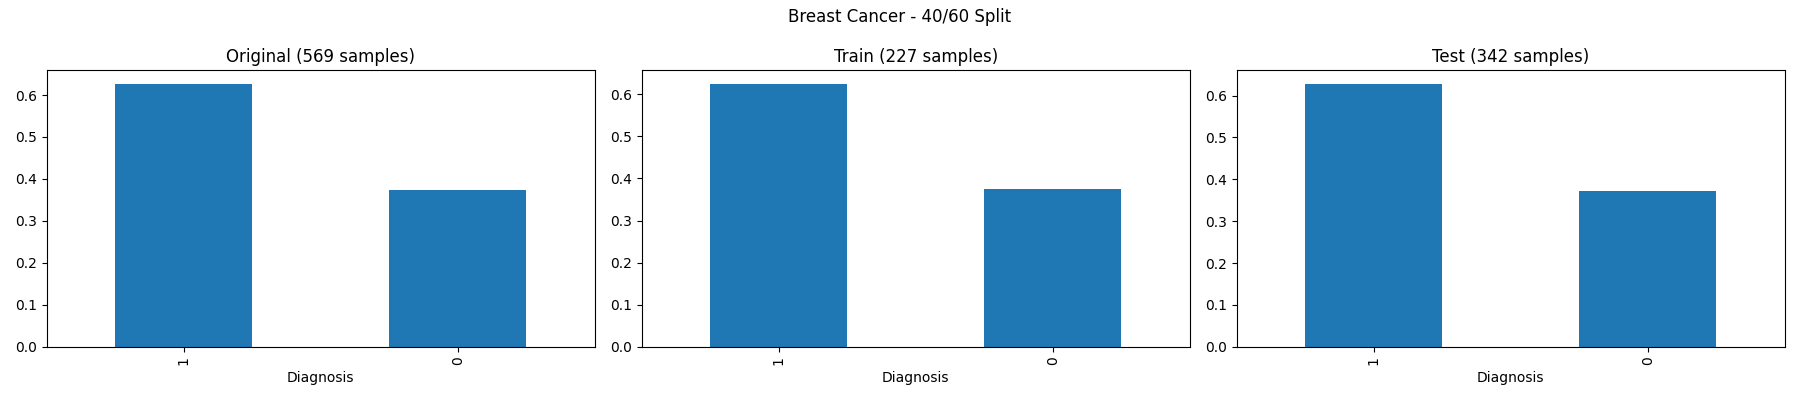
\includegraphics[width=0.6\textwidth]{imgs/class_dist/class_dist__breast_cancer__40_vs_60.png}
	\caption{Breast Cancer: class distribution (40/60 split).}
	\label{fig:bc-cd-40-60}
\end{figure}

\begin{figure}[H]
	\centering
	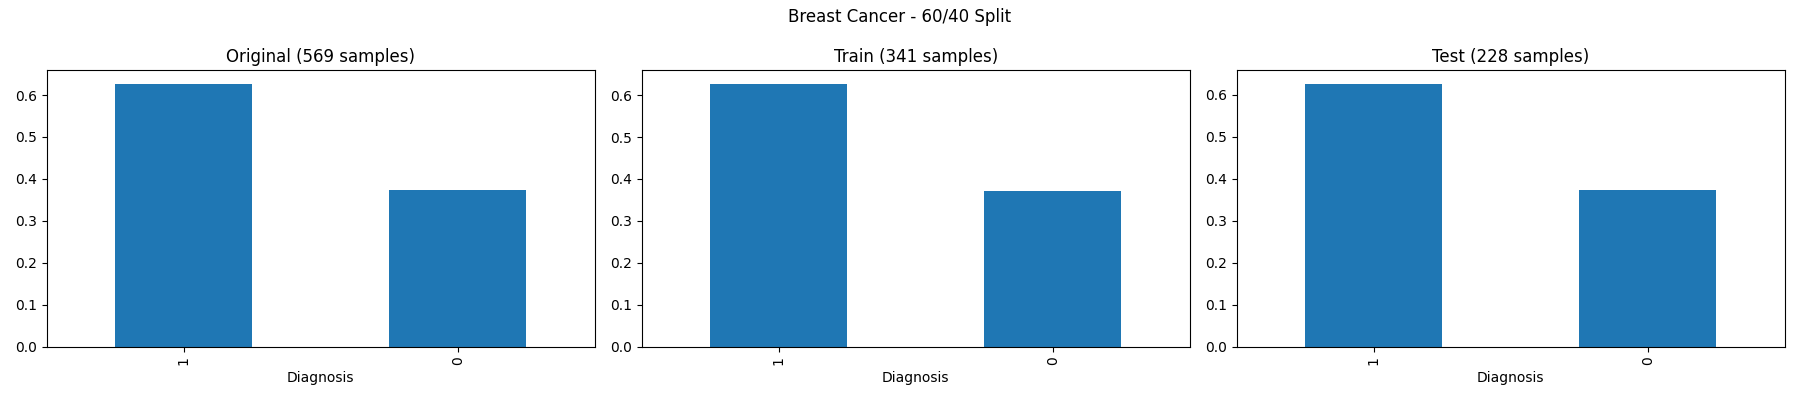
\includegraphics[width=0.6\textwidth]{imgs/class_dist/class_dist__breast_cancer__60_vs_40.png}
	\caption{Breast Cancer: class distribution (60/40 split).}
	\label{fig:bc-cd-60-40}
\end{figure}

\begin{figure}[H]
	\centering
	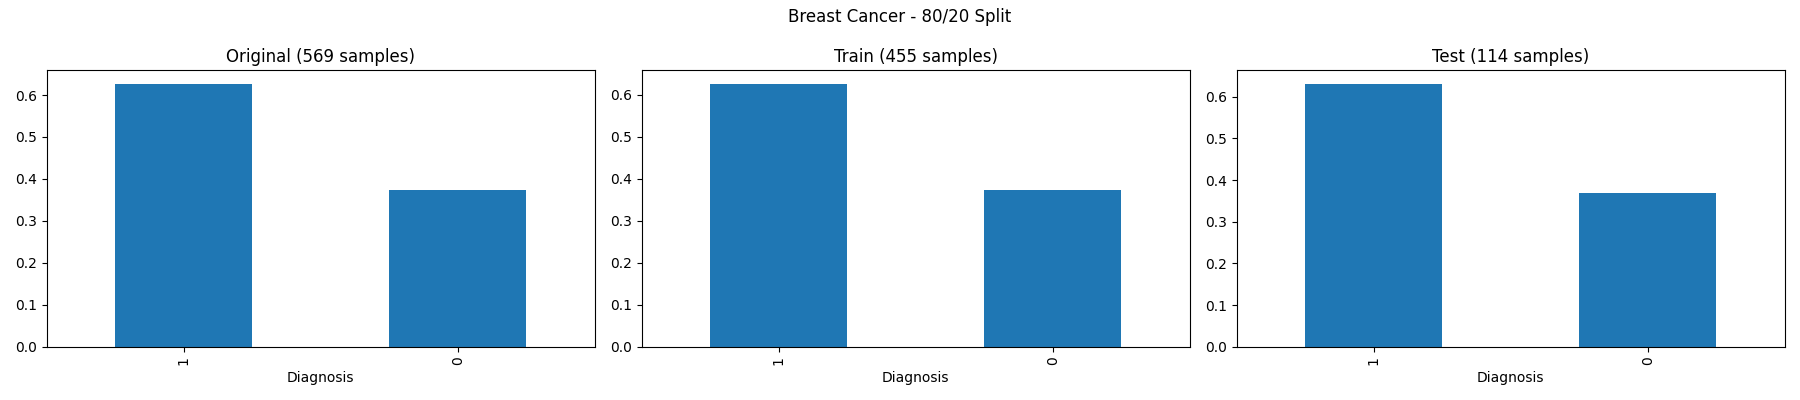
\includegraphics[width=0.6\textwidth]{imgs/class_dist/class_dist__breast_cancer__80_vs_20.png}
	\caption{Breast Cancer: class distribution (80/20 split).}
	\label{fig:bc-cd-80-20}
\end{figure}

\begin{figure}[H]
	\centering
	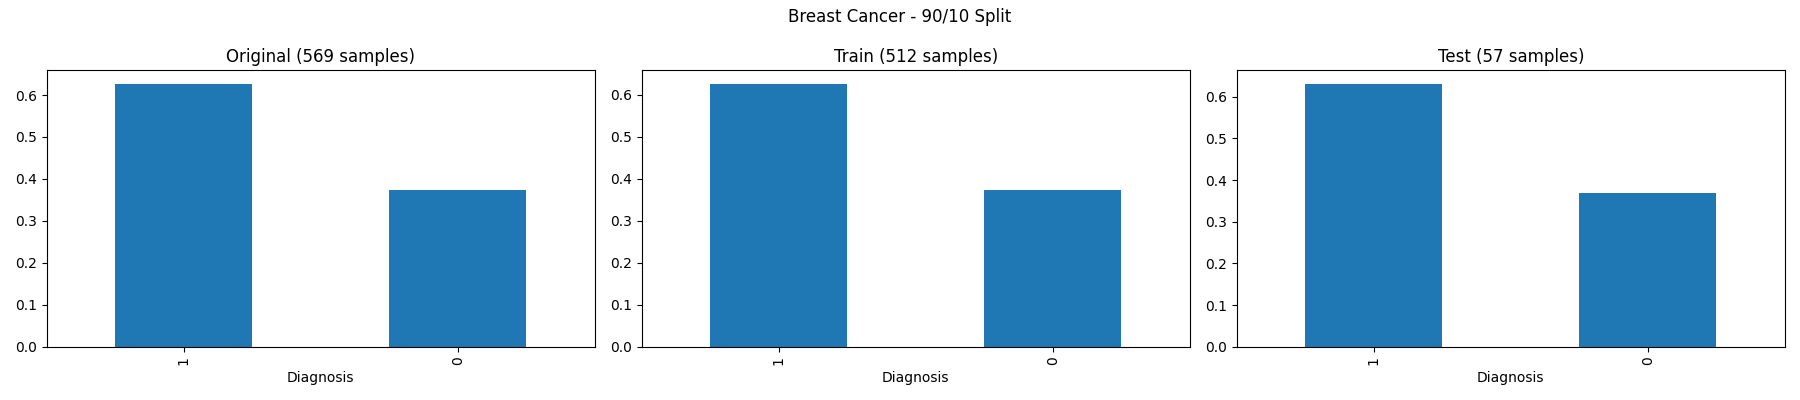
\includegraphics[width=0.6\textwidth]{imgs/class_dist/class_dist__breast_cancer__90_vs_10.png}
	\caption{Breast Cancer: class distribution (90/10 split).}
	\label{fig:bc-cd-90-10}
\end{figure}

\begin{figure}[H]
	\centering
	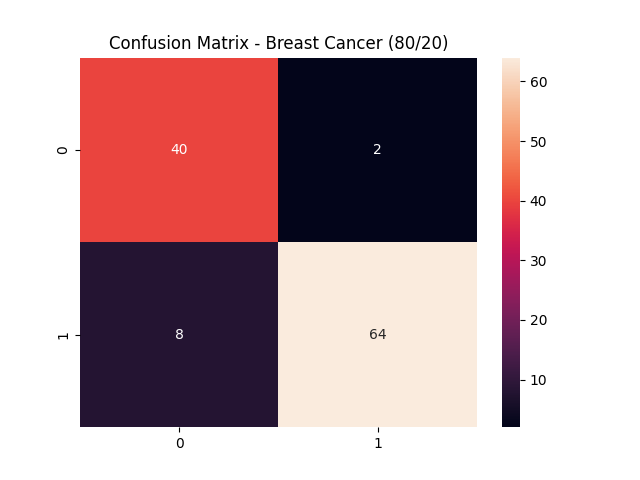
\includegraphics[width=0.6\textwidth]{imgs/confusion_mat/confusion_mat__breast_cancer__80_vs_20.png}
	\caption{Breast Cancer: confusion matrix (80/20 split).}
	\label{fig:bc-cm-80-20}
\end{figure}

\begin{figure}[H]
	\centering
	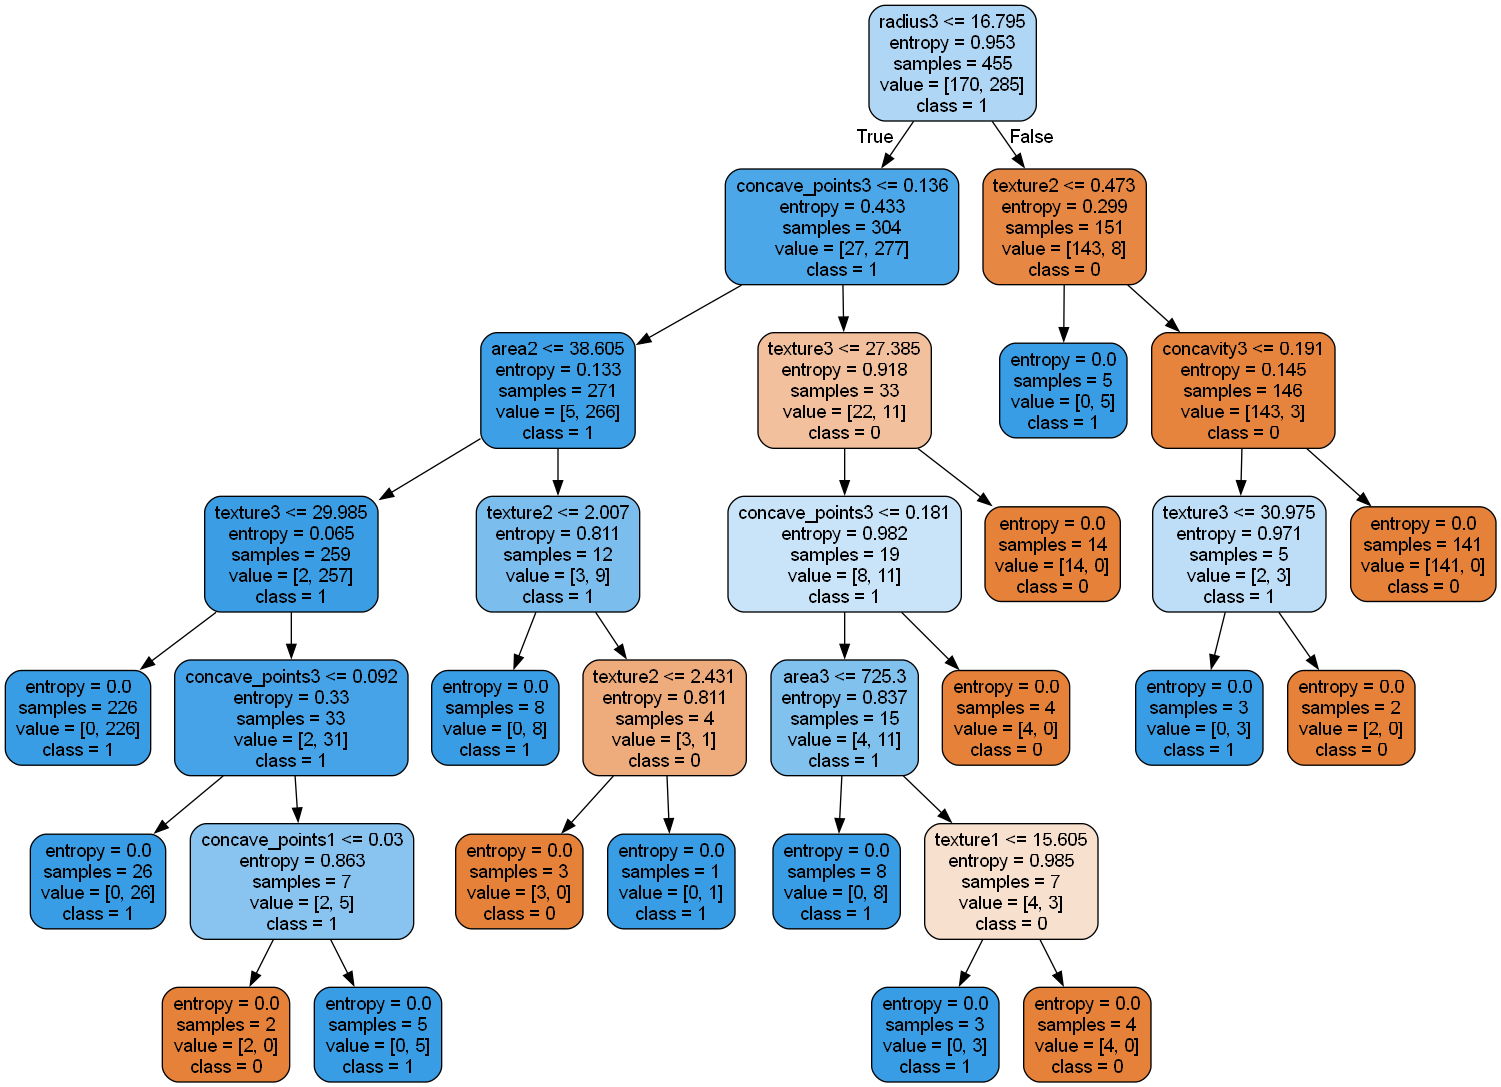
\includegraphics[width=0.8\textwidth]{imgs/dt/dt__breast_cancer__80_vs_20.png}
	\caption{Breast Cancer: decision tree (base) for 80/20 split.}
	\label{fig:bc-dt-base}
\end{figure}

\begin{figure}[H]
	\centering
	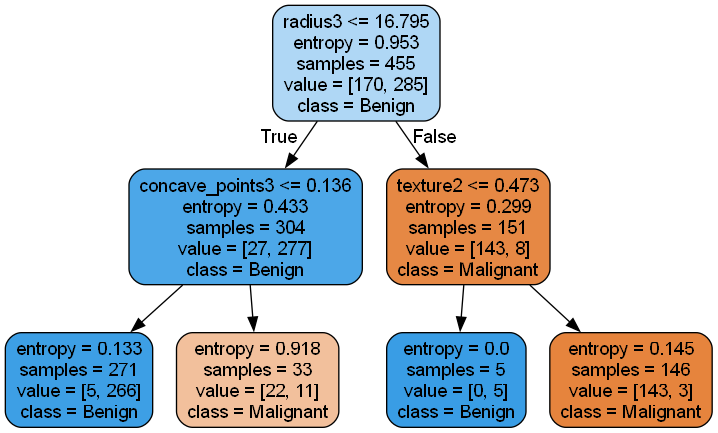
\includegraphics[width=0.8\textwidth]{imgs/dt/dt__breast_cancer__80_vs_20__2.png}
	\caption{Breast Cancer: decision tree with \texttt{max\_depth}=2 (80/20 split).}
	\label{fig:bc-dt-depth-2}
\end{figure}

\begin{figure}[H]
	\centering
	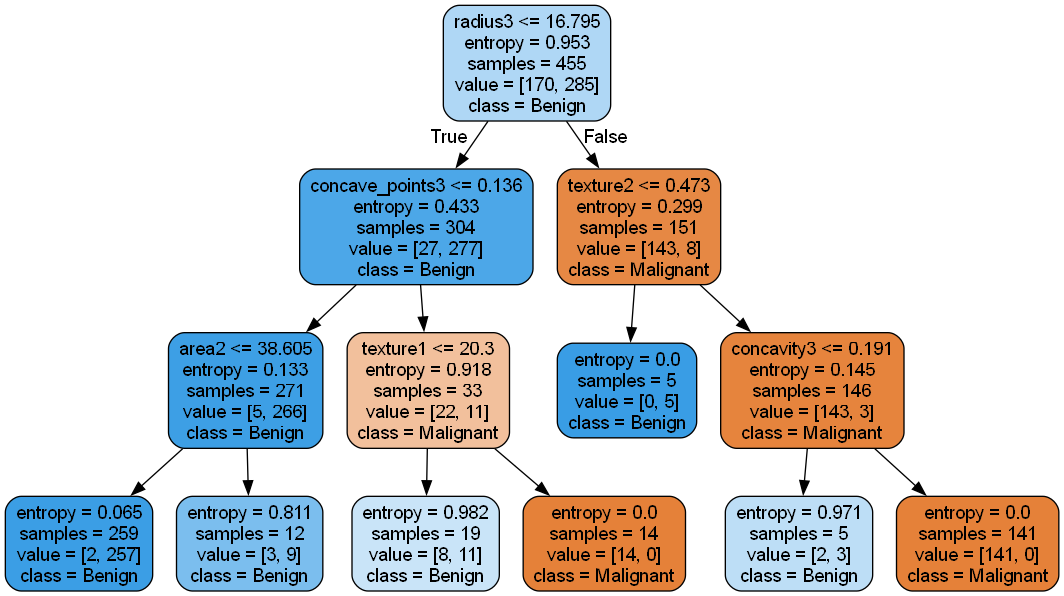
\includegraphics[width=0.8\textwidth]{imgs/dt/dt__breast_cancer__80_vs_20__3.png}
	\caption{Breast Cancer: decision tree with \texttt{max\_depth}=3 (80/20 split).}
	\label{fig:bc-dt-depth-3}
\end{figure}

\begin{figure}[H]
	\centering
	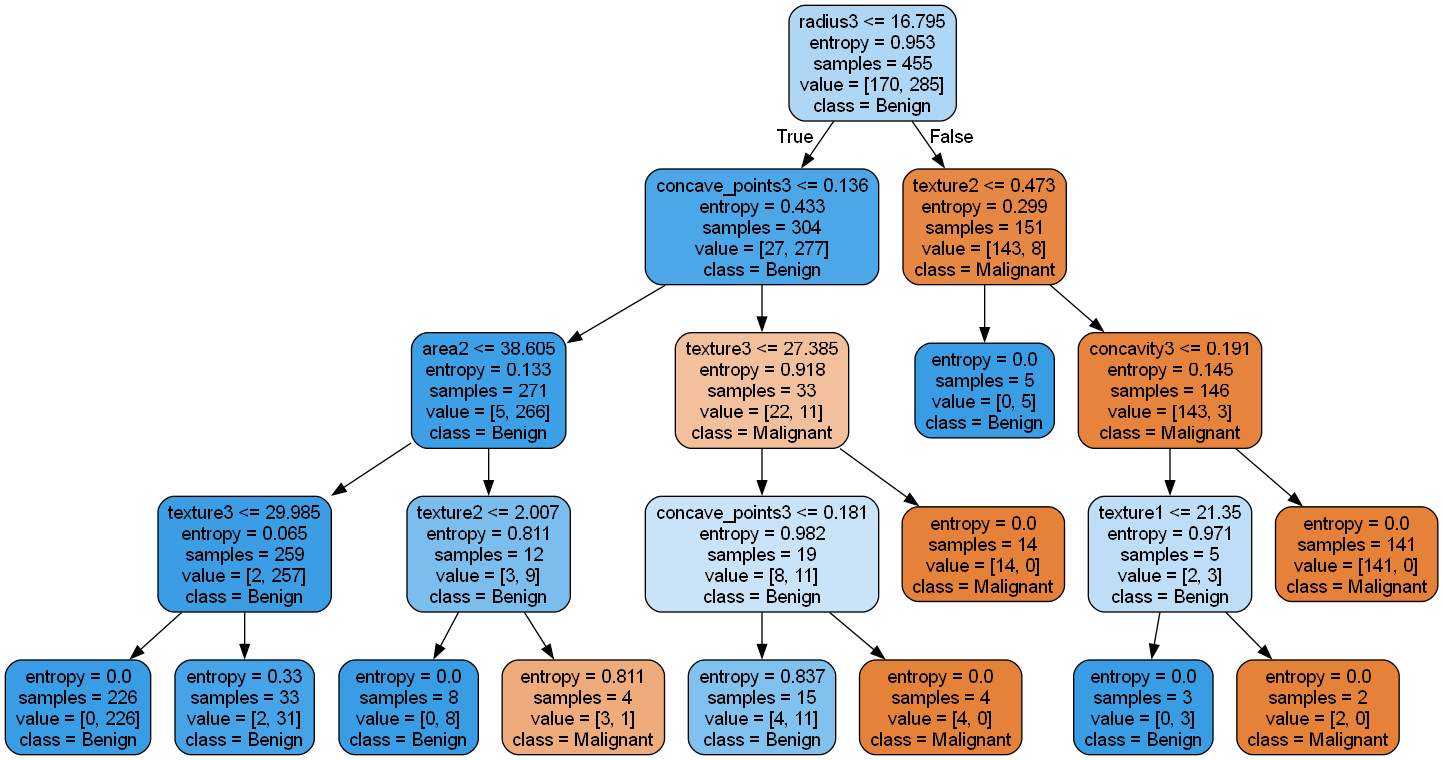
\includegraphics[width=0.8\textwidth]{imgs/dt/dt__breast_cancer__80_vs_20__4.png}
	\caption{Breast Cancer: decision tree with \texttt{max\_depth}=4 (80/20 split).}
	\label{fig:bc-dt-depth-4}
\end{figure}

\begin{figure}[H]
	\centering
	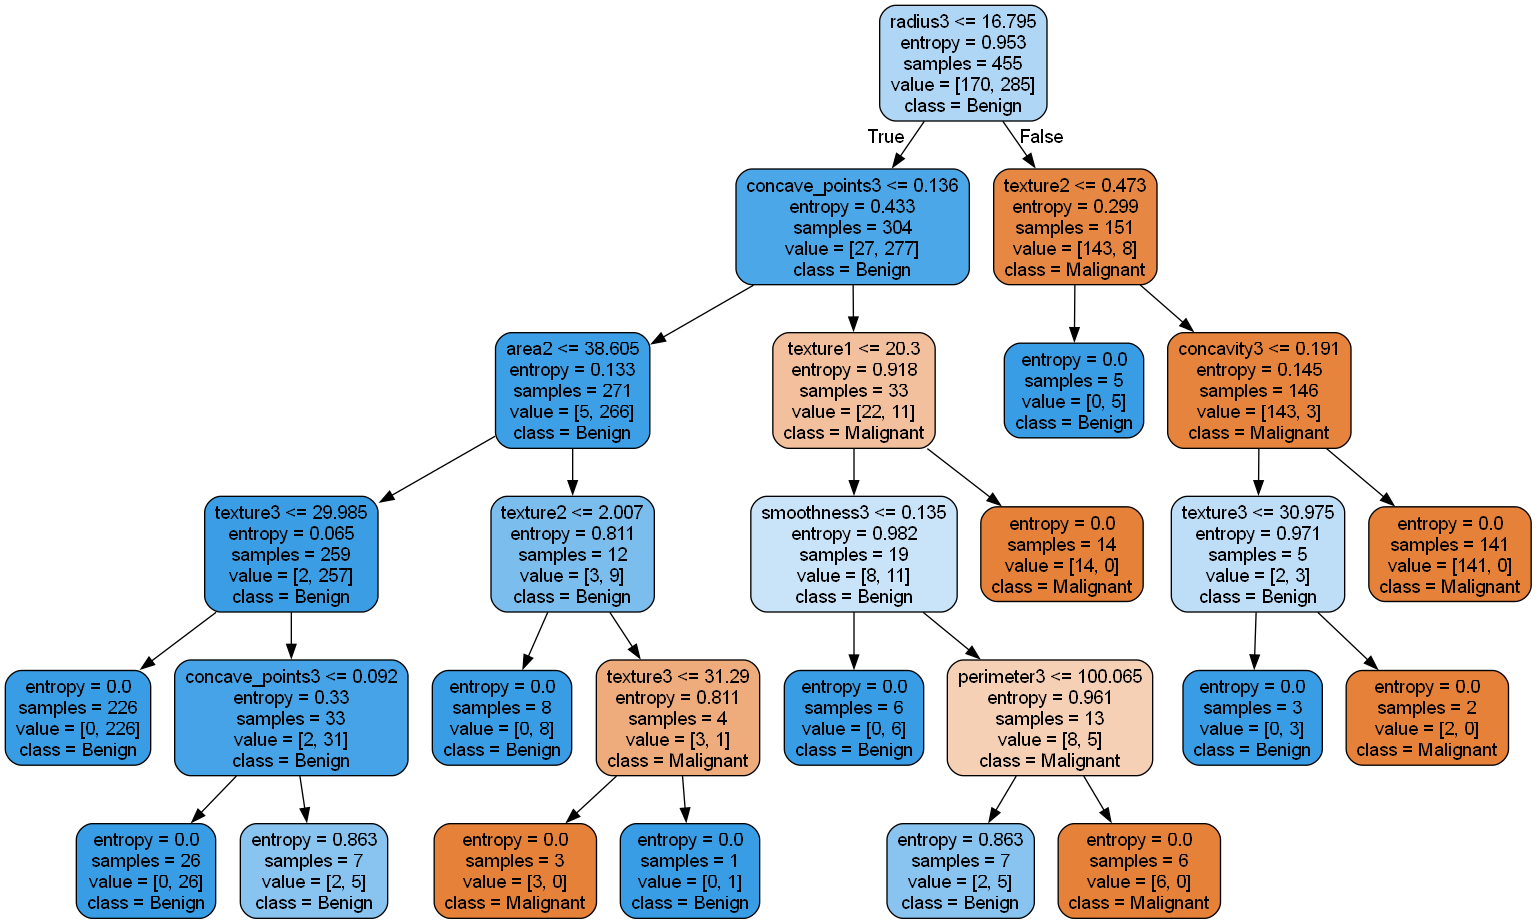
\includegraphics[width=0.8\textwidth]{imgs/dt/dt__breast_cancer__80_vs_20__5.png}
	\caption{Breast Cancer: decision tree with \texttt{max\_depth}=5 (80/20 split).}
	\label{fig:bc-dt-depth-5}
\end{figure}

\begin{figure}[H]
	\centering
	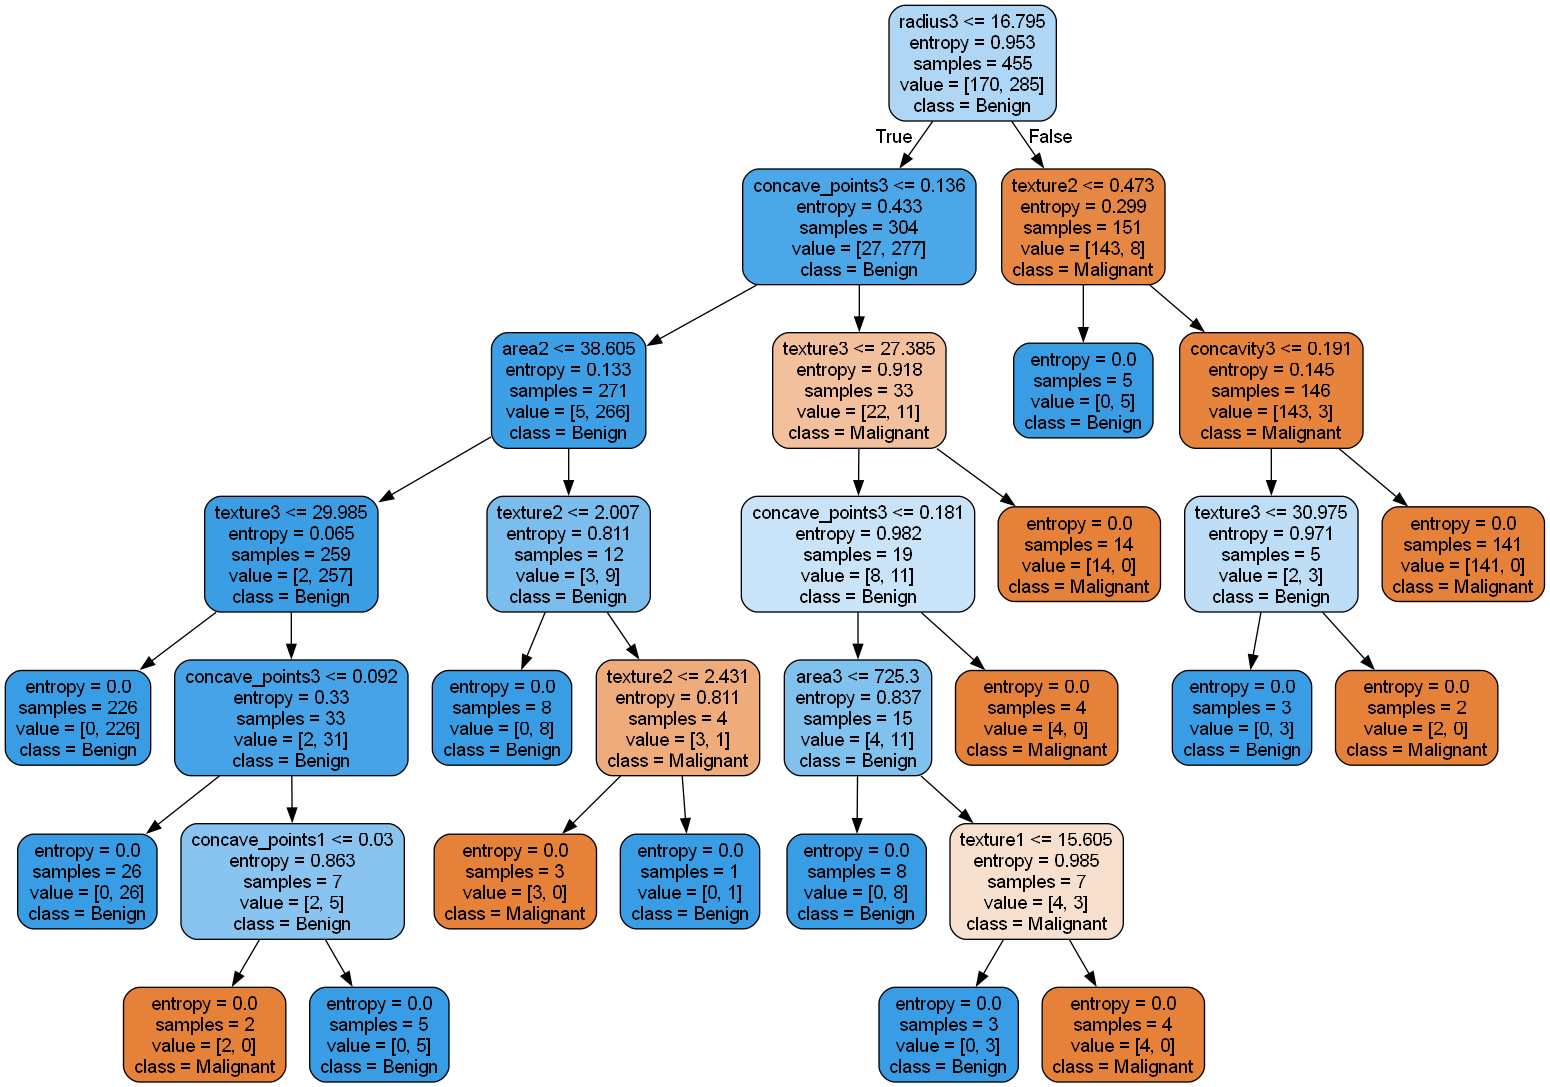
\includegraphics[width=0.8\textwidth]{imgs/dt/dt__breast_cancer__80_vs_20__6.png}
	\caption{Breast Cancer: decision tree with \texttt{max\_depth}=6 (80/20 split).}
	\label{fig:bc-dt-depth-6}
\end{figure}

\begin{figure}[H]
	\centering
	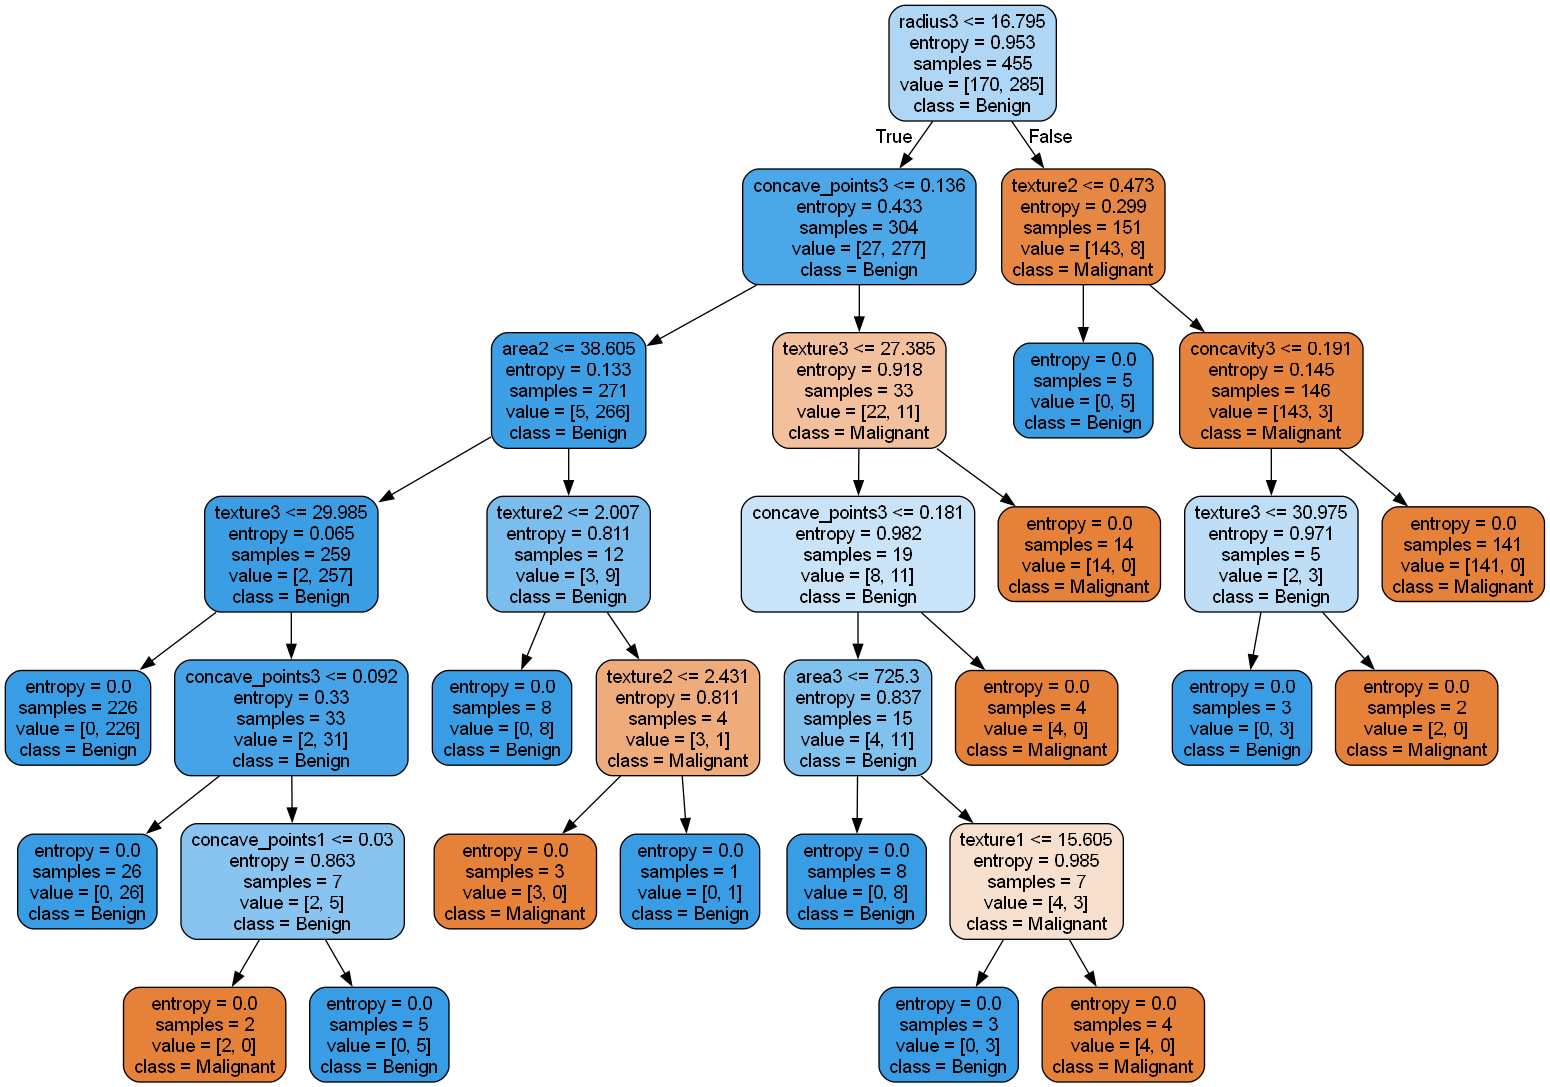
\includegraphics[width=0.8\textwidth]{imgs/dt/dt__breast_cancer__80_vs_20__7.png}
	\caption{Breast Cancer: decision tree with \texttt{max\_depth}=7 (80/20 split).}
	\label{fig:bc-dt-depth-7}
\end{figure}

\begin{figure}[H]
	\centering
	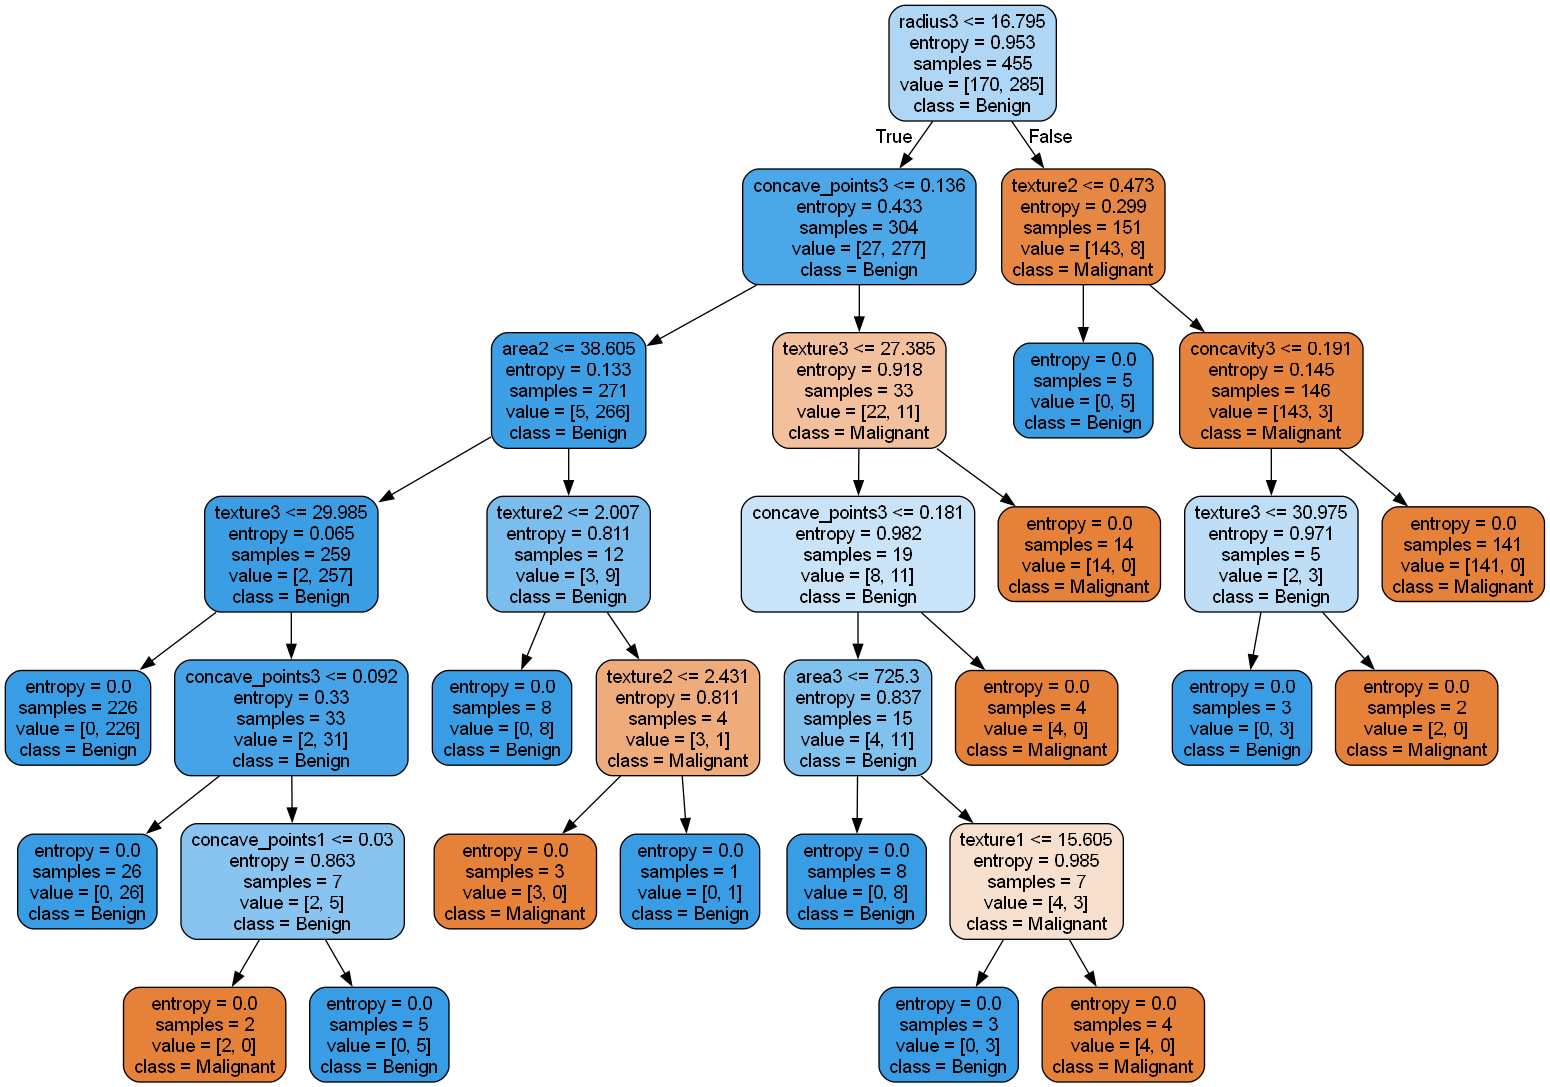
\includegraphics[width=0.8\textwidth]{imgs/dt/dt__breast_cancer__80_vs_20__None.png}
	\caption{Breast Cancer: decision tree with \texttt{max\_depth}=None (80/20 split).}
	\label{fig:bc-dt-depth-none}
\end{figure}

\clearpage

%================ Wine Quality =================%
\subsection{Wine Quality Dataset}
\begin{itemize}
	\item \textbf{Description:} 4,898 samples; original scores 0–10 grouped into Low (0–4), Standard (5–6), High (7–10).
	\item \textbf{Preprocessing:} label encoding, stratified splits at 40/60, 60/40, 80/20, 90/10.
\end{itemize}

\begin{figure}[H]
	\centering
	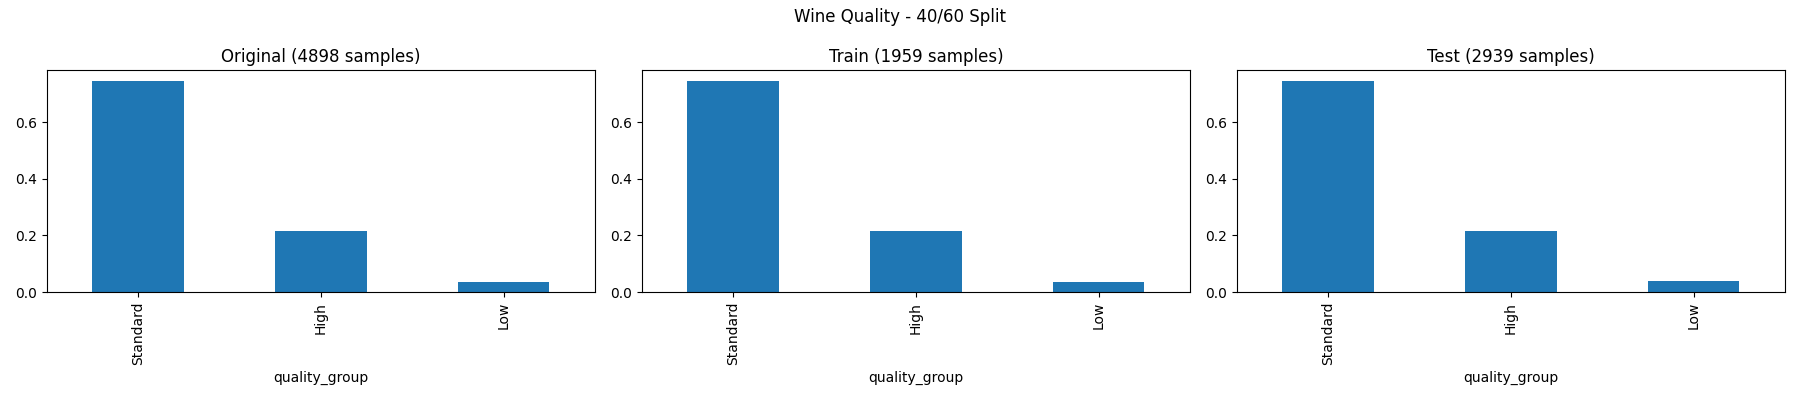
\includegraphics[width=0.6\textwidth]{imgs/class_dist/class_dist__wine_quality__40_vs_60.png}
	\caption{Wine Quality: class distribution (40/60 split).}
	\label{fig:wq-cd-40-60}
\end{figure}

\begin{figure}[H]
	\centering
	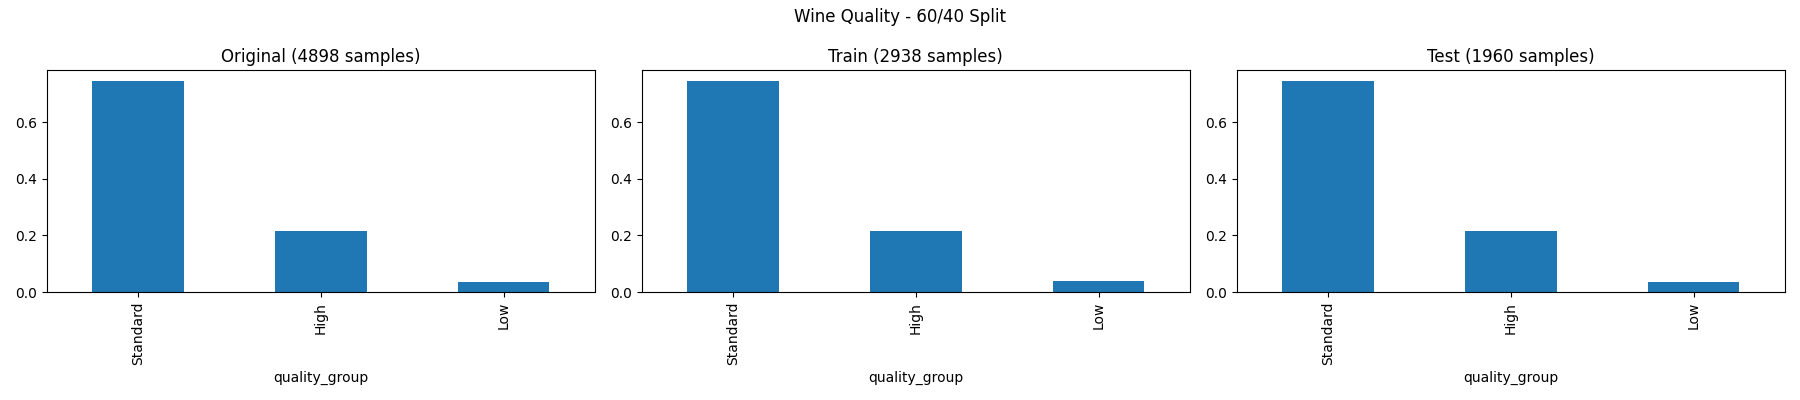
\includegraphics[width=0.6\textwidth]{imgs/class_dist/class_dist__wine_quality__60_vs_40.png}
	\caption{Wine Quality: class distribution (60/40 split).}
	\label{fig:wq-cd-60-40}
\end{figure}

\begin{figure}[H]
	\centering
	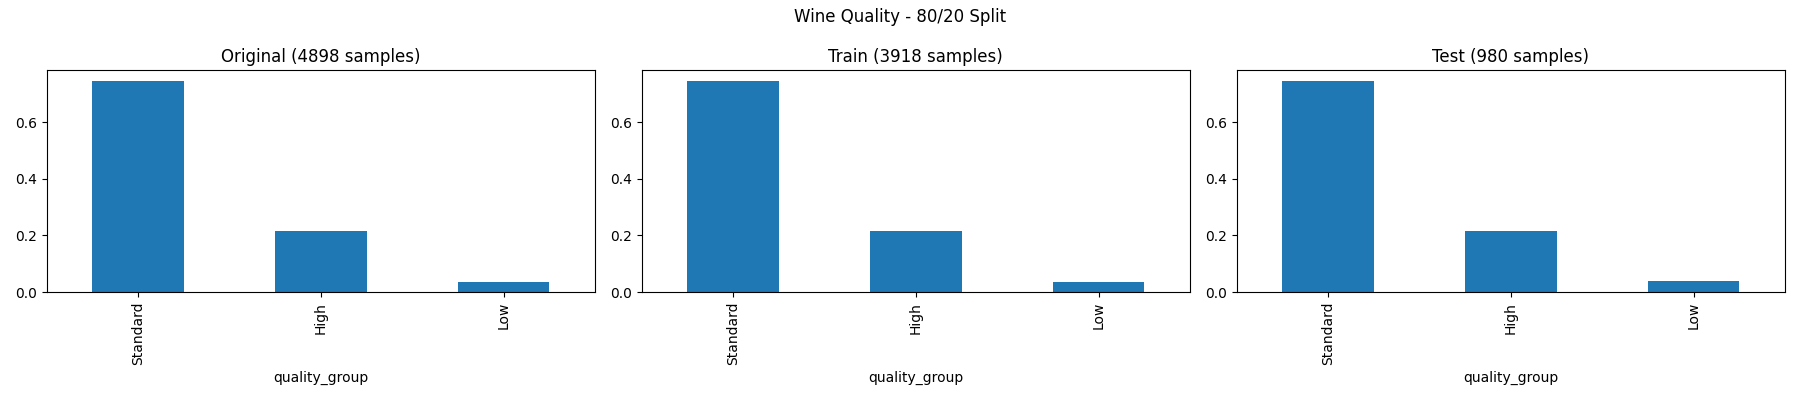
\includegraphics[width=0.6\textwidth]{imgs/class_dist/class_dist__wine_quality__80_vs_20.png}
	\caption{Wine Quality: class distribution (80/20 split).}
	\label{fig:wq-cd-80-20}
\end{figure}

\begin{figure}[H]
	\centering
	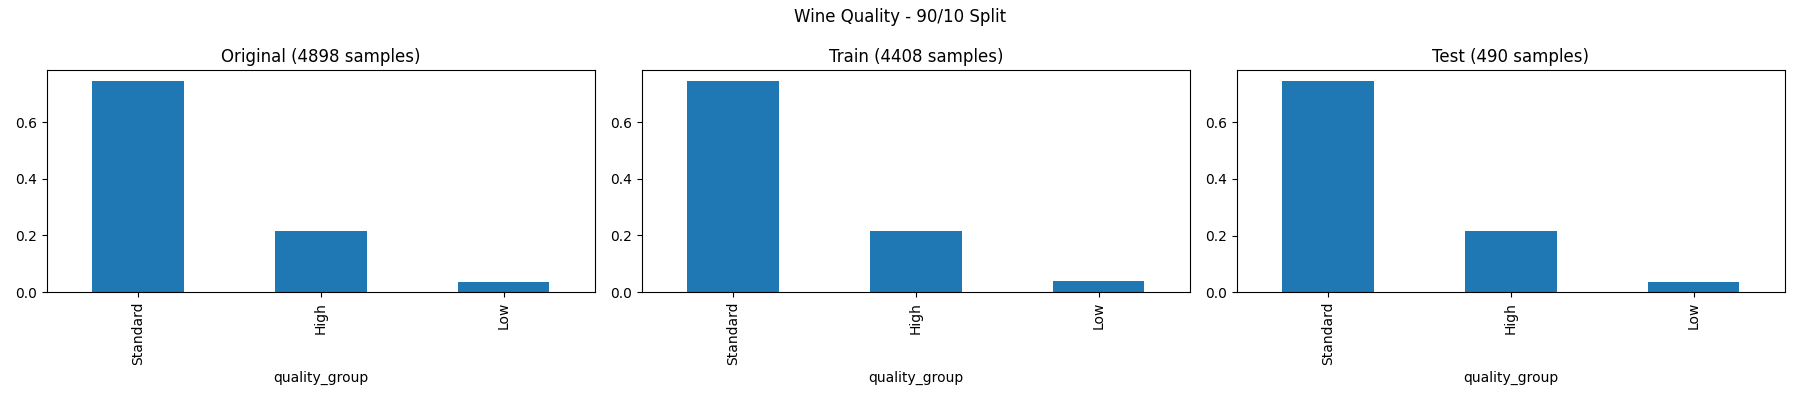
\includegraphics[width=0.6\textwidth]{imgs/class_dist/class_dist__wine_quality__90_vs_10.png}
	\caption{Wine Quality: class distribution (90/10 split).}
	\label{fig:wq-cd-90-10}
\end{figure}

\begin{figure}[H]
	\centering
	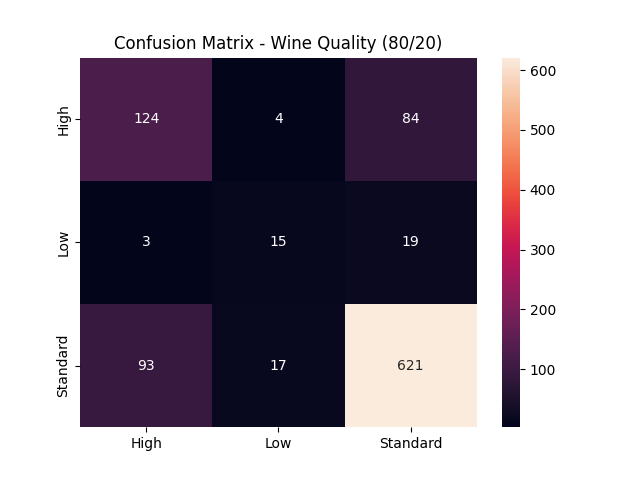
\includegraphics[width=0.6\textwidth]{imgs/confusion_mat/confusion_mat__wine_quality__80_vs_20.png}
	\caption{Wine Quality: confusion matrix (80/20 split).}
	\label{fig:wq-cm-80-20}
\end{figure}

\begin{figure}[H]
	\centering
	% \includegraphics[width=0.8\textwidth]{imgs/dt/dt__wine_quality__80_vs_20.png}
	\caption{Wine Quality: decision tree (base) for 80/20 split.}
	\label{fig:wq-dt-base}
\end{figure}

\begin{figure}[H]
	\centering
	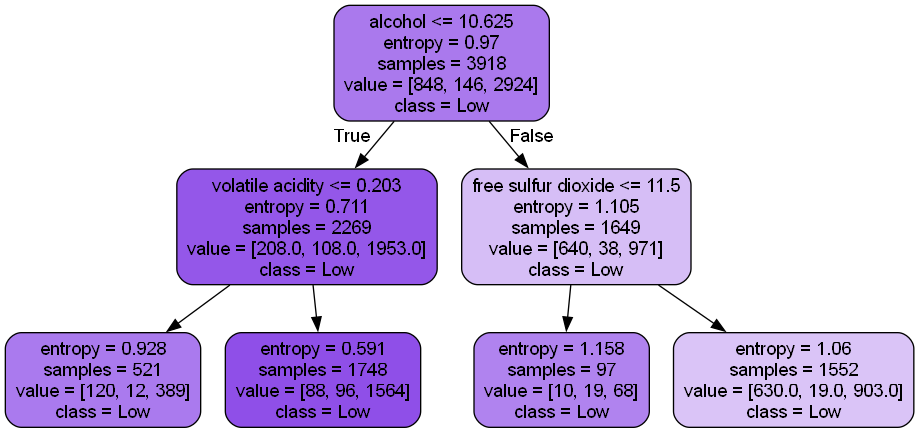
\includegraphics[width=0.8\textwidth]{imgs/dt/dt__wine_quality__80_vs_20__2.png}
	\caption{Wine Quality: decision tree with \texttt{max\_depth}=2 (80/20 split).}
	\label{fig:wq-dt-depth-2}
\end{figure}

\begin{figure}[H]
	\centering
	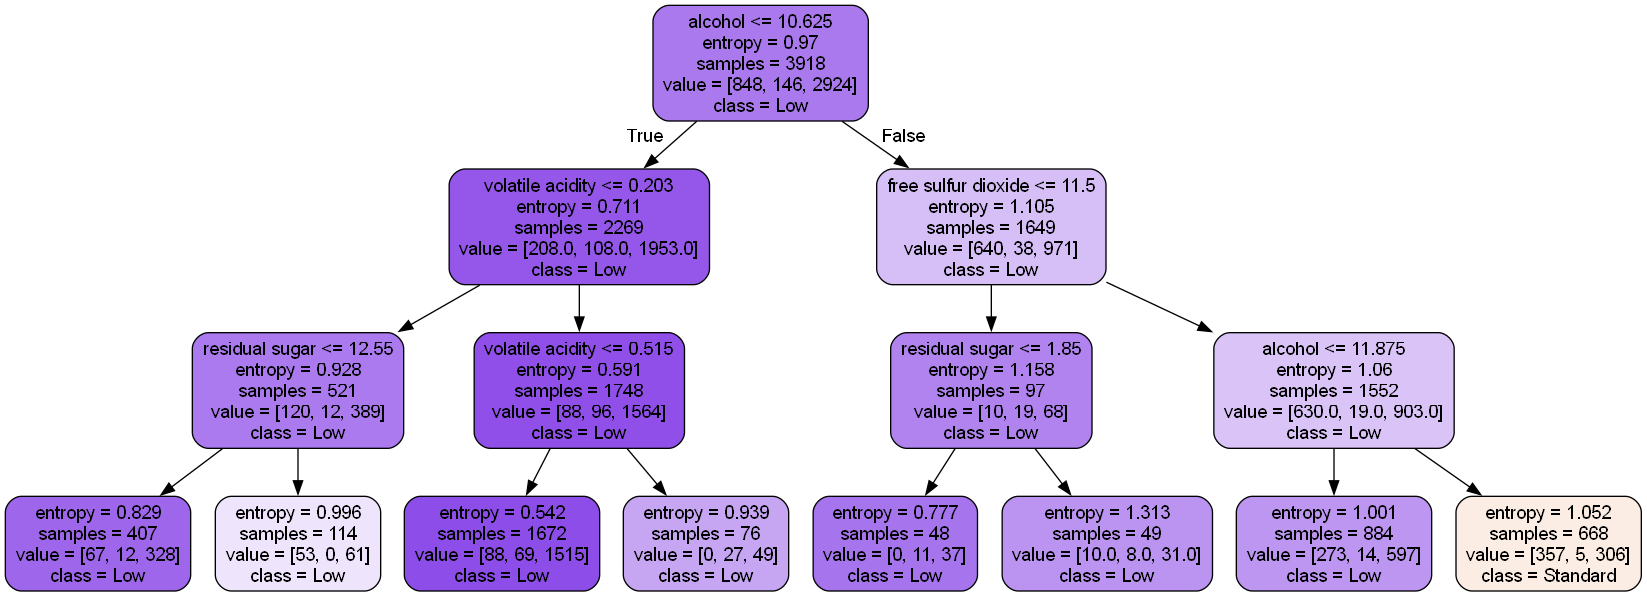
\includegraphics[width=0.8\textwidth]{imgs/dt/dt__wine_quality__80_vs_20__3.png}
	\caption{Wine Quality: decision tree with \texttt{max\_depth}=3 (80/20 split).}
	\label{fig:wq-dt-depth-3}
\end{figure}

\begin{figure}[H]
	\centering
	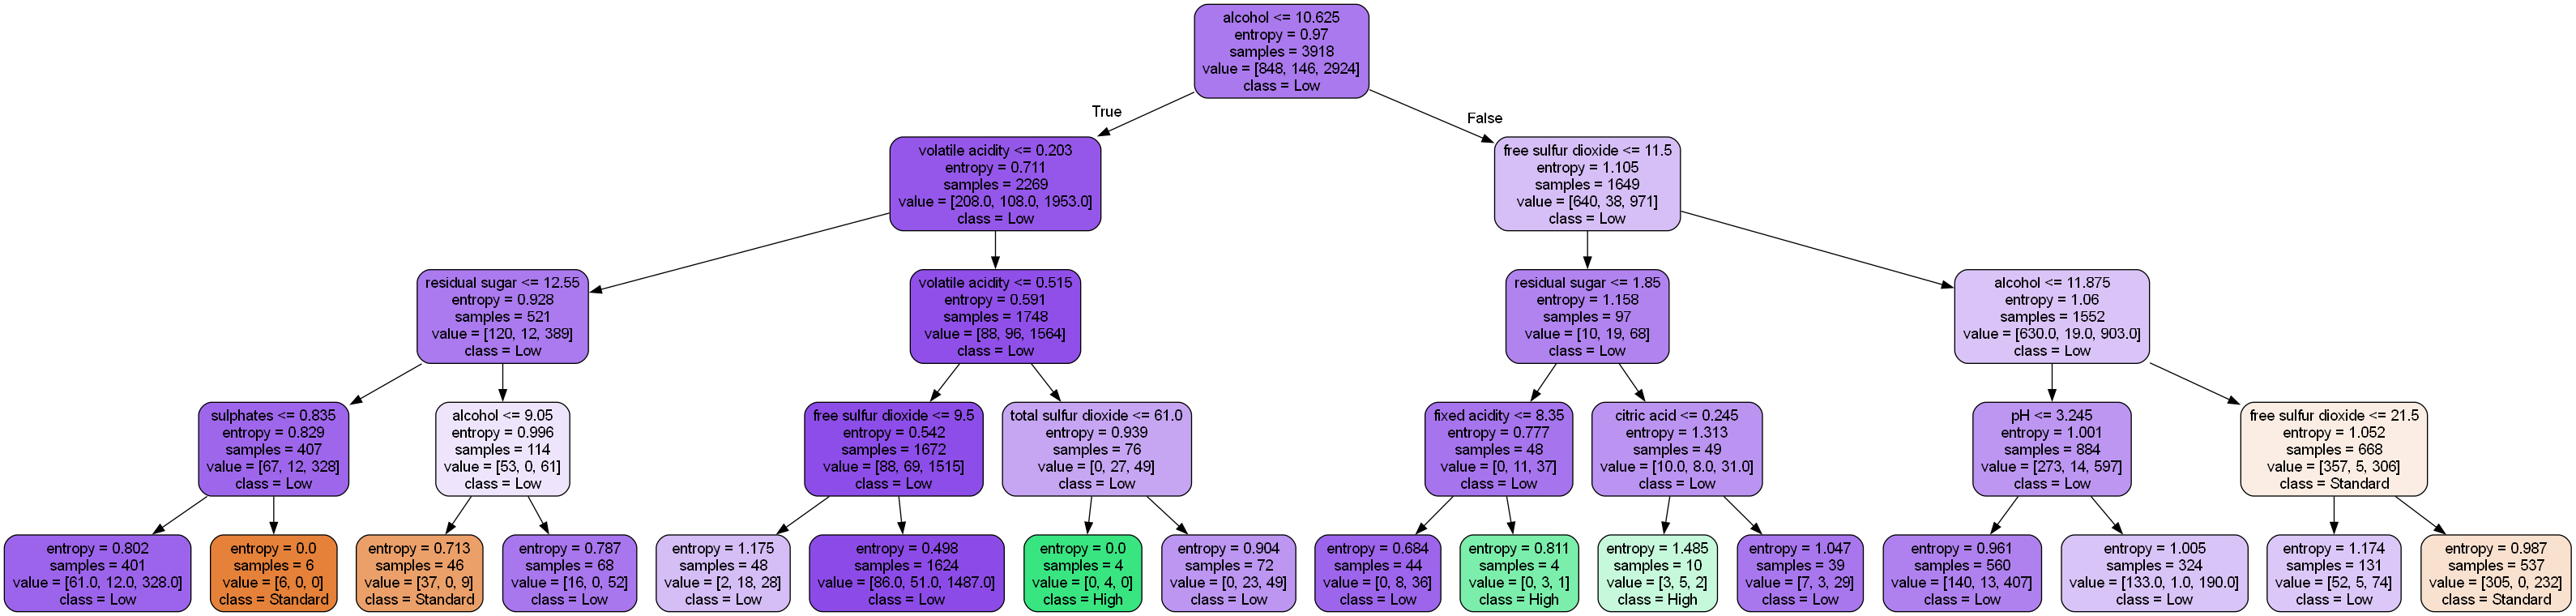
\includegraphics[width=0.8\textwidth]{imgs/dt/dt__wine_quality__80_vs_20__4.png}
	\caption{Wine Quality: decision tree with \texttt{max\_depth}=4 (80/20 split).}
	\label{fig:wq-dt-depth-4}
\end{figure}

\begin{figure}[H]
	\centering
	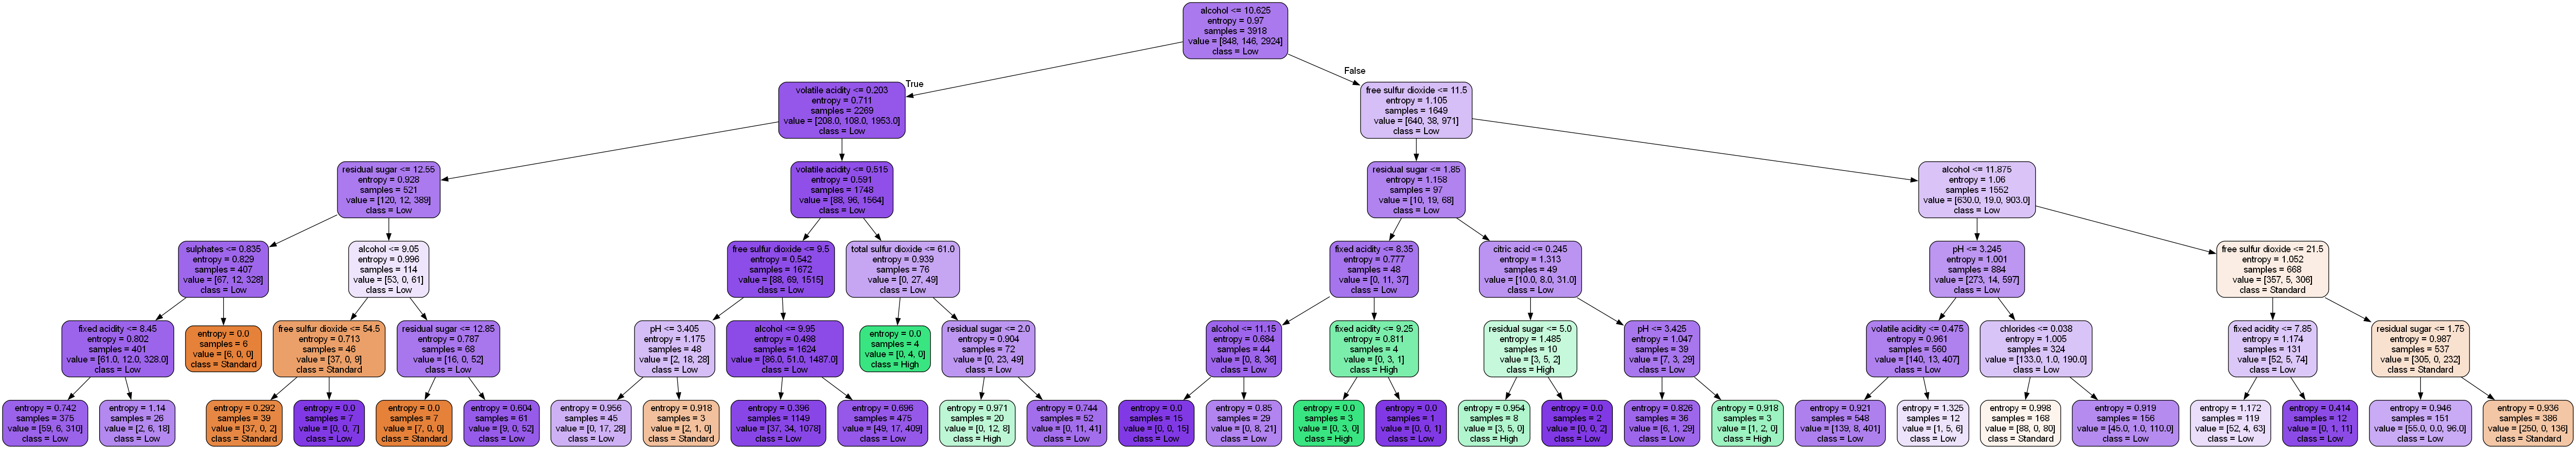
\includegraphics[width=0.8\textwidth]{imgs/dt/dt__wine_quality__80_vs_20__5.png}
	\caption{Wine Quality: decision tree with \texttt{max\_depth}=5 (80/20 split).}
	\label{fig:wq-dt-depth-5}
\end{figure}

\begin{figure}[H]
	\centering
	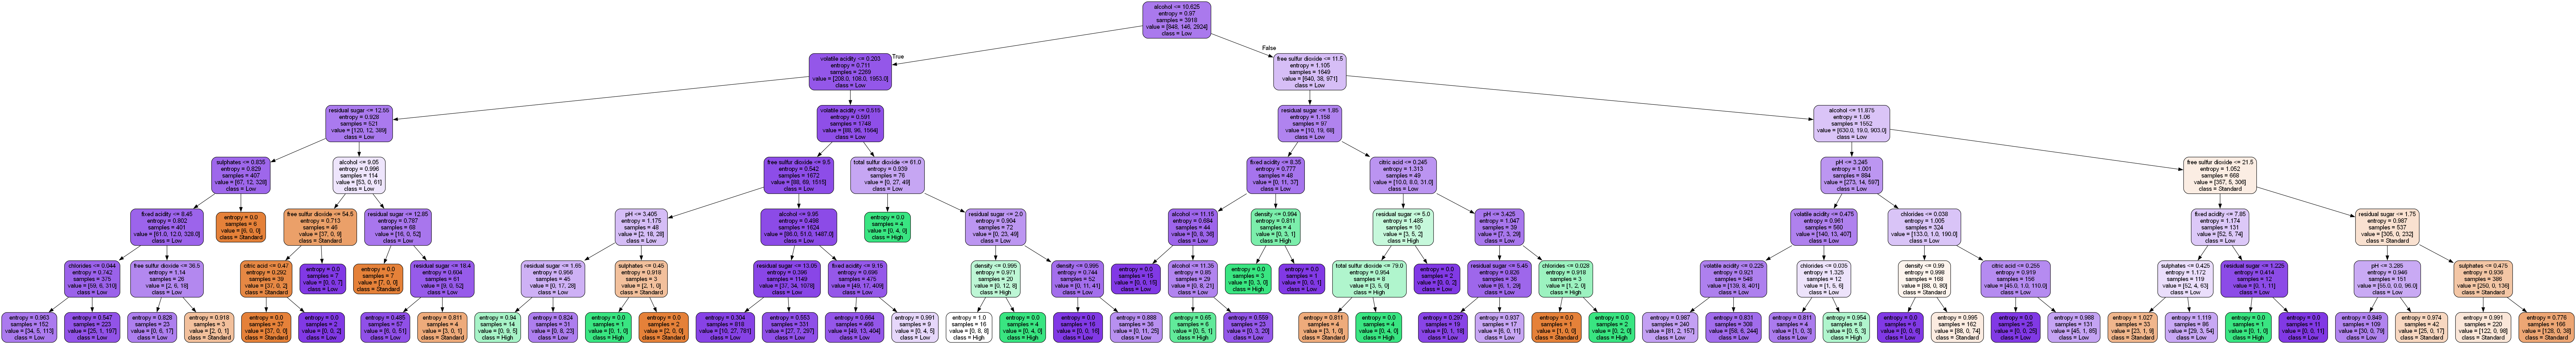
\includegraphics[width=0.8\textwidth]{imgs/dt/dt__wine_quality__80_vs_20__6.png}
	\caption{Wine Quality: decision tree with \texttt{max\_depth}=6 (80/20 split).}
	\label{fig:wq-dt-depth-6}
\end{figure}

\begin{figure}[H]
	\centering
	
\includegraphics[width=0.8\textwidth]{imgs/dt/dt__wine_quality__80_vs_20__7.png}
	\caption{Wine Quality: decision tree with \texttt{max\_depth}=7 (80/20 split).}
	\label{fig:wq-dt-depth-7}
\end{figure}

\begin{figure}[H]
	\centering
	% \includegraphics[width=0.8\textwidth]{imgs/dt/dt__wine_quality__80_vs_20__None.png}
	\caption{Wine Quality: decision tree with \texttt{max\_depth}=None (80/20 split).}
	\label{fig:wq-dt-depth-none}
\end{figure}

\clearpage

%================ Car Evaluation =================%
\subsection{Car Evaluation Dataset}
\begin{itemize}
	\item \textbf{Description:} 1,728 samples; 4 classes (\texttt{unacc}, \texttt{acc}, \texttt{good}, \texttt{vgood}), 6 categorical features.
	\item \textbf{Preprocessing:} label encoding, stratified splits at 40/60, 60/40, 80/20, 90/10.
\end{itemize}

\begin{figure}[H]
	\centering
	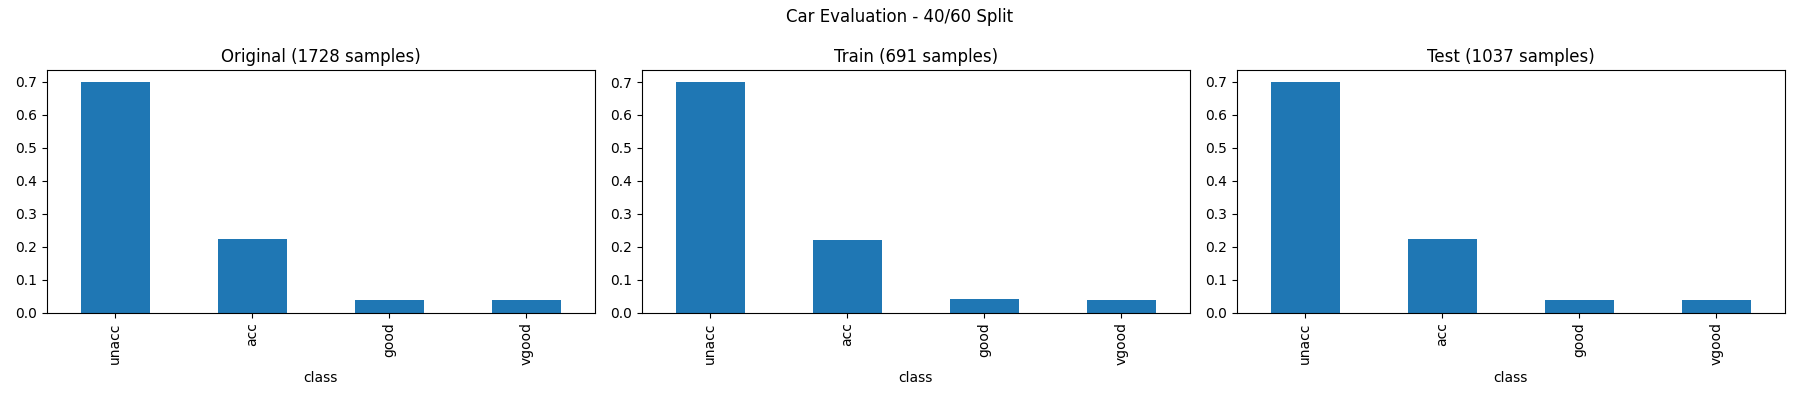
\includegraphics[width=0.6\textwidth]{imgs/class_dist/class_dist__car_evaluation__40_vs_60.png}
	\caption{Car Evaluation: class distribution (40/60 split).}
	\label{fig:ce-cd-40-60}
\end{figure}

\begin{figure}[H]
	\centering
	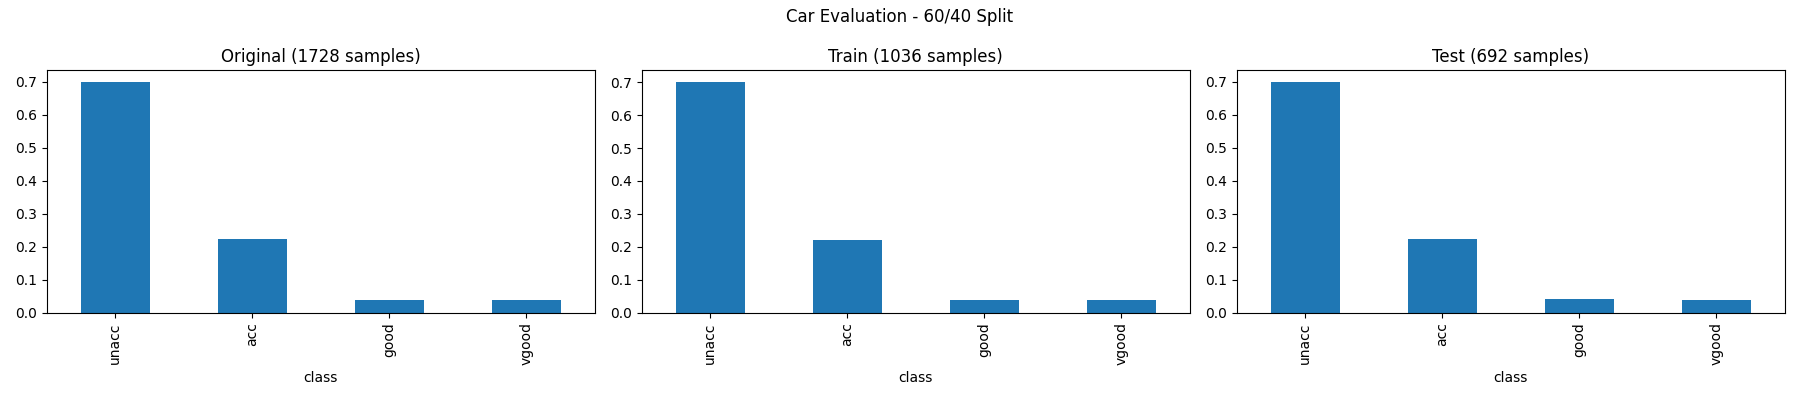
\includegraphics[width=0.6\textwidth]{imgs/class_dist/class_dist__car_evaluation__60_vs_40.png}
	\caption{Car Evaluation: class distribution (60/40 split).}
	\label{fig:ce-cd-60-40}
\end{figure}

\begin{figure}[H]
	\centering
	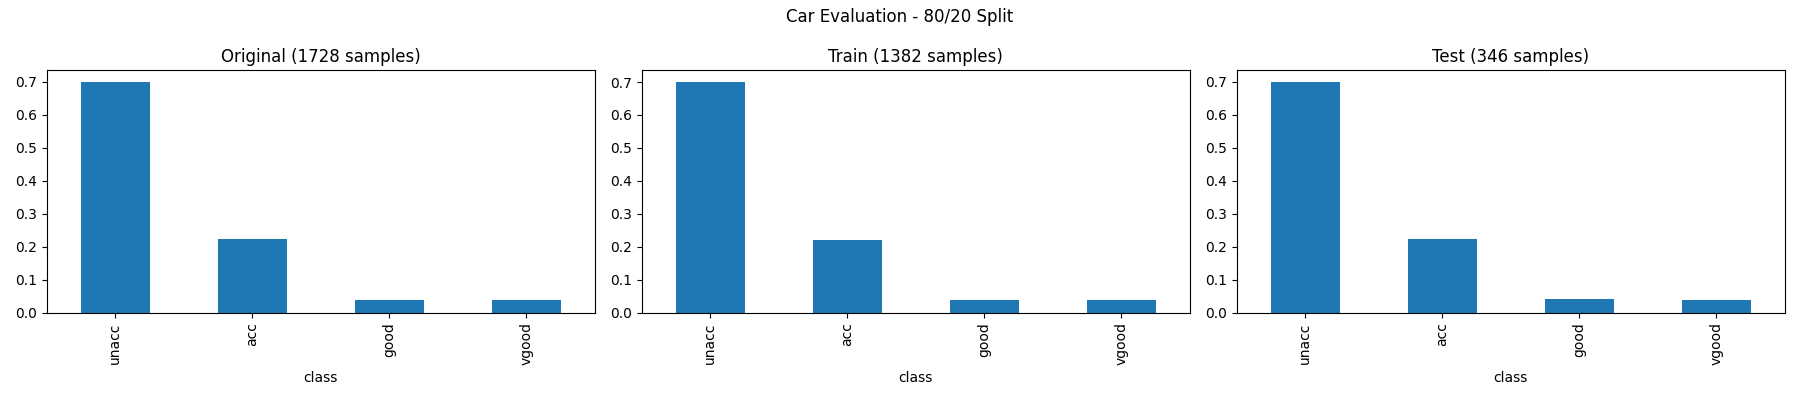
\includegraphics[width=0.6\textwidth]{imgs/class_dist/class_dist__car_evaluation__80_vs_20.png}
	\caption{Car Evaluation: class distribution (80/20 split).}
	\label{fig:ce-cd-80-20}
\end{figure}

\begin{figure}[H]
	\centering
	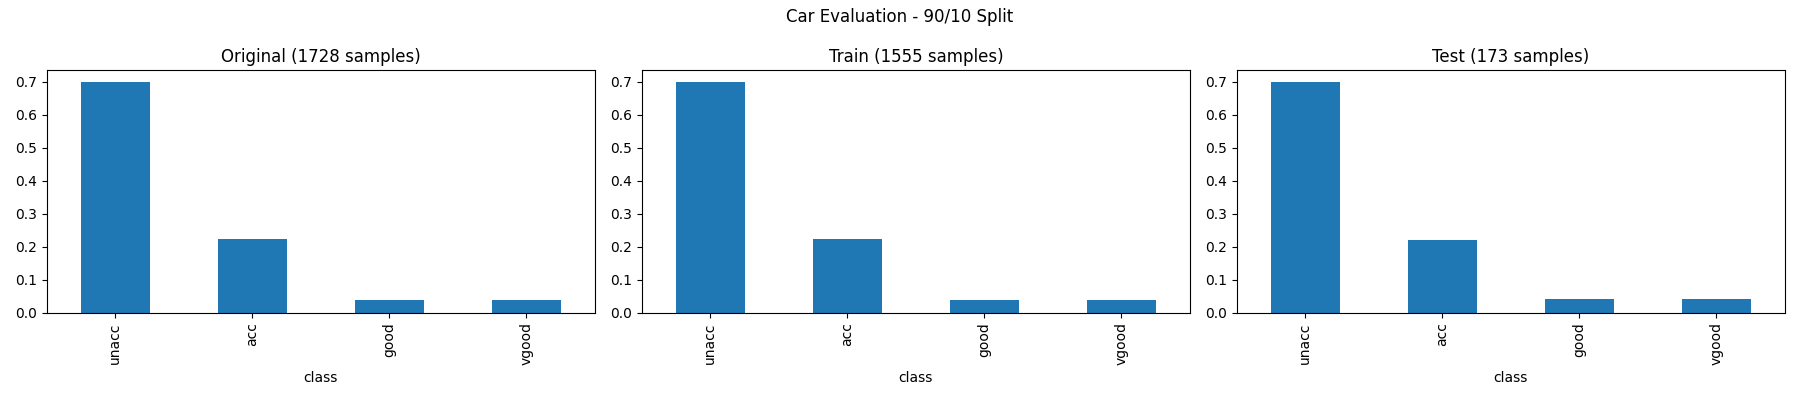
\includegraphics[width=0.6\textwidth]{imgs/class_dist/class_dist__car_evaluation__90_vs_10.png}
	\caption{Car Evaluation: class distribution (90/10 split).}
	\label{fig:ce-cd-90-10}
\end{figure}

\begin{figure}[H]
	\centering
	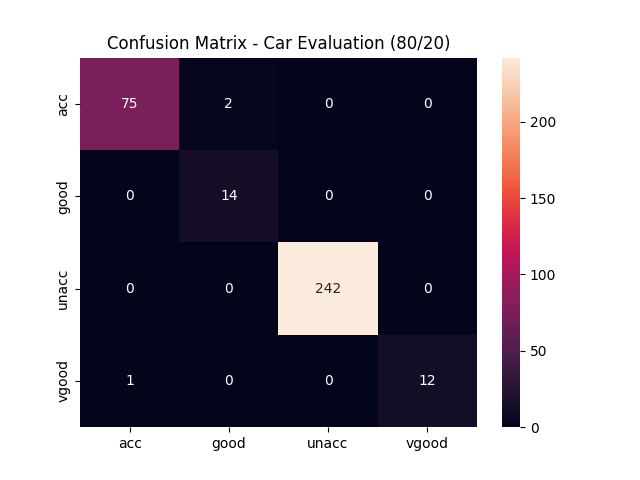
\includegraphics[width=0.6\textwidth]{imgs/confusion_mat/confusion_mat__car_evaluation__80_vs_20.png}
	\caption{Car Evaluation: confusion matrix (80/20 split).}
	\label{fig:ce-cm-80-20}
\end{figure}

\begin{figure}[H]
	\centering
	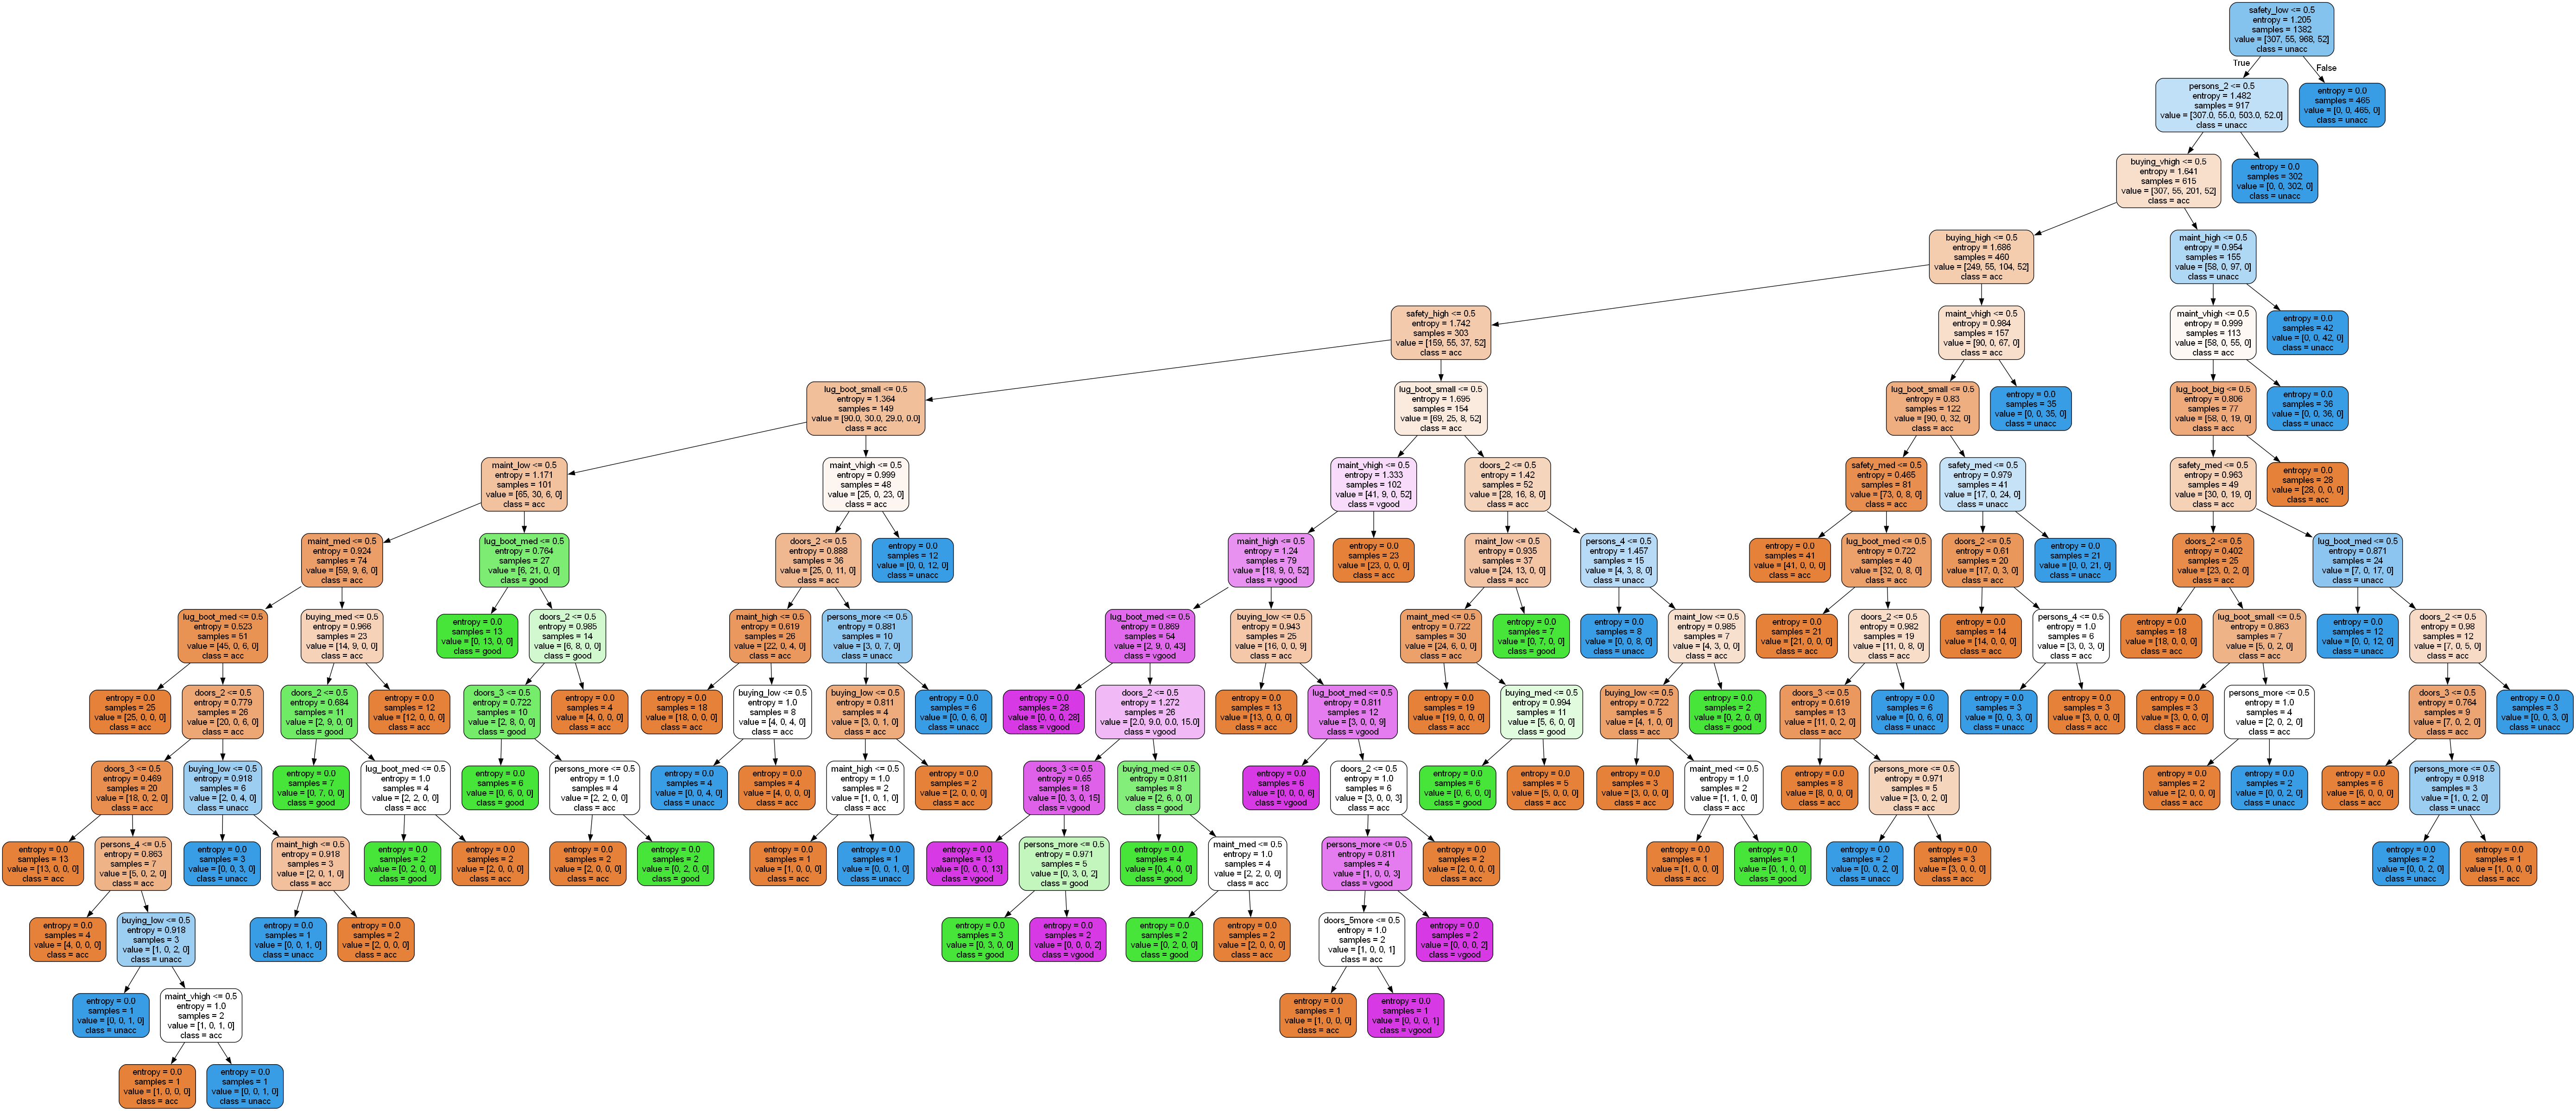
\includegraphics[width=0.8\textwidth]{imgs/dt/dt__car_evaluation__80_vs_20.png}
	\caption{Car Evaluation: decision tree (base) for 80/20 split.}
	\label{fig:ce-dt-base}
\end{figure}

\begin{figure}[H]
	\centering
	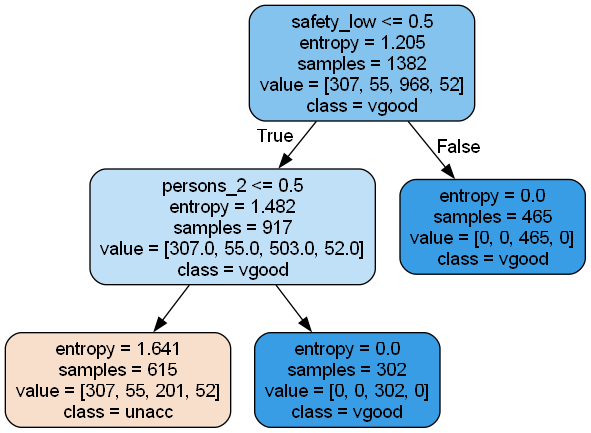
\includegraphics[width=0.8\textwidth]{imgs/dt/dt__car_evaluation__80_vs_20__2.png}
	\caption{Car Evaluation: decision tree with \texttt{max\_depth}=2 (80/20 split).}
	\label{fig:ce-dt-depth-2}
\end{figure}

\begin{figure}[H]
	\centering
	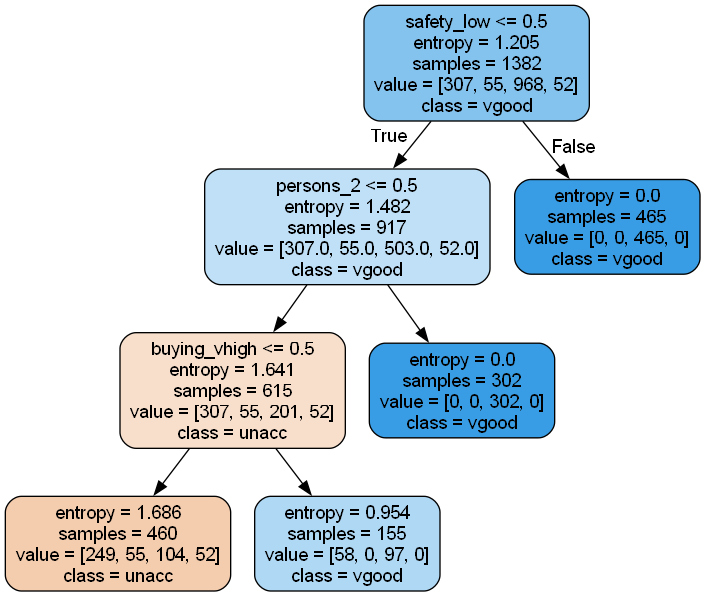
\includegraphics[width=0.8\textwidth]{imgs/dt/dt__car_evaluation__80_vs_20__3.png}
	\caption{Car Evaluation: decision tree with \texttt{max\_depth}=3 (80/20 split).}
	\label{fig:ce-dt-depth-3}
\end{figure}

\begin{figure}[H]
	\centering
	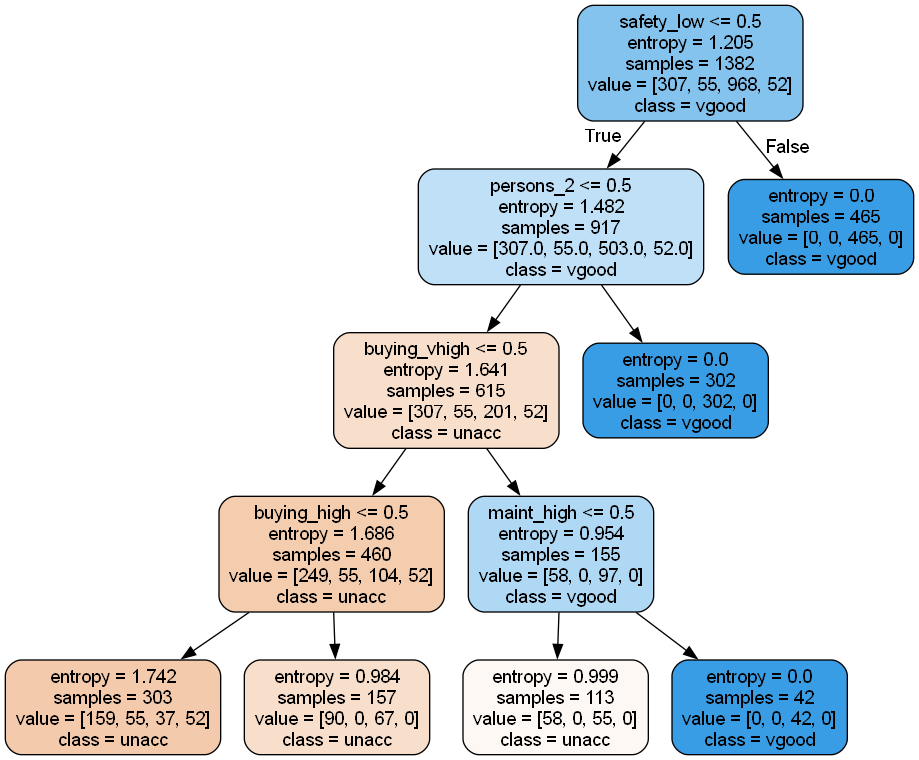
\includegraphics[width=0.8\textwidth]{imgs/dt/dt__car_evaluation__80_vs_20__4.png}
	\caption{Car Evaluation: decision tree with \texttt{max\_depth}=4 (80/20 split).}
	\label{fig:ce-dt-depth-4}
\end{figure}

\begin{figure}[H]
	\centering
	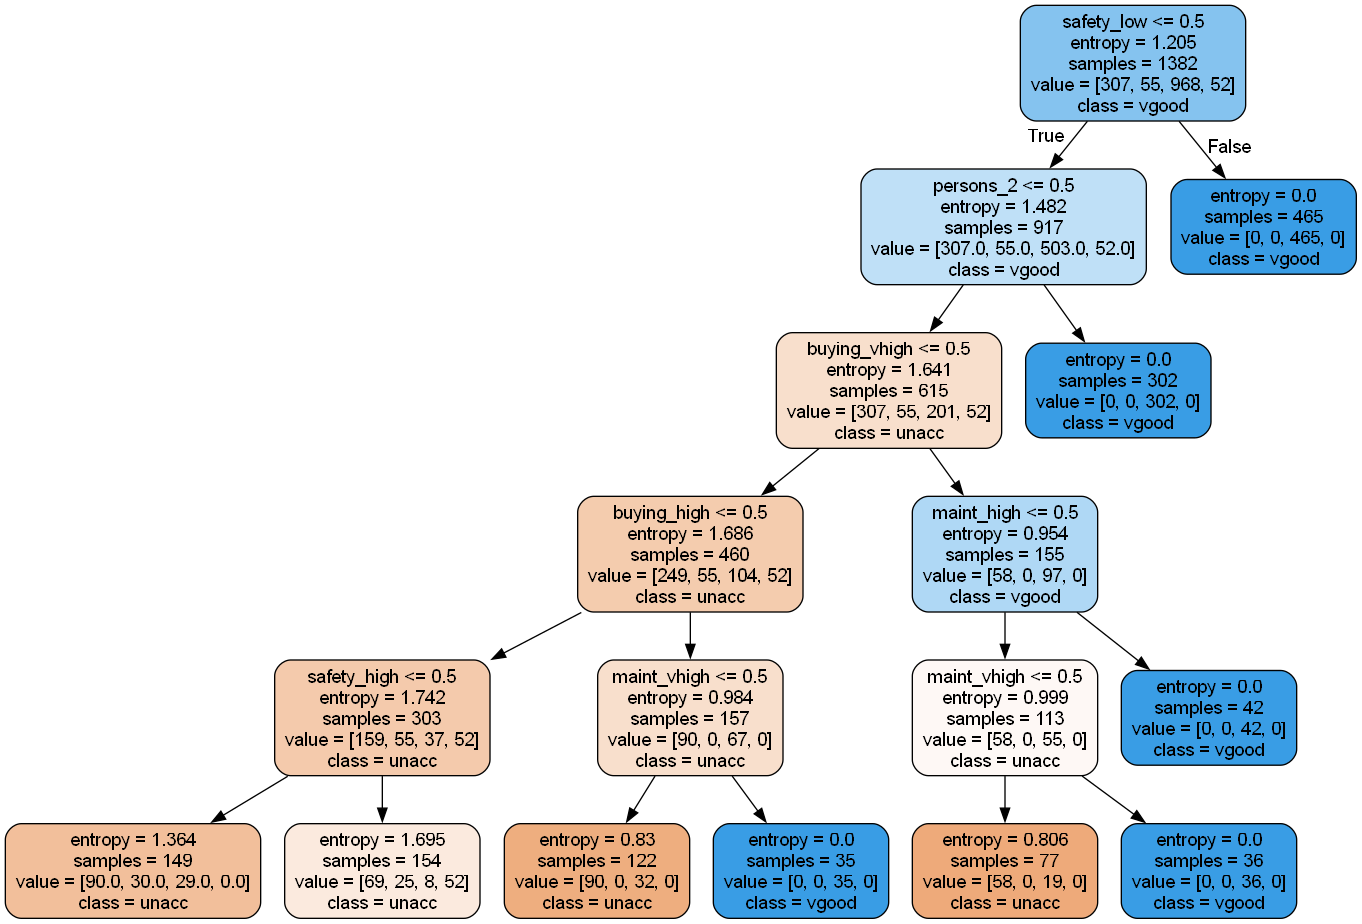
\includegraphics[width=0.8\textwidth]{imgs/dt/dt__car_evaluation__80_vs_20__5.png}
	\caption{Car Evaluation: decision tree with \texttt{max\_depth}=5 (80/20 split).}
	\label{fig:ce-dt-depth-5}
\end{figure}

\begin{figure}[H]
	\centering
	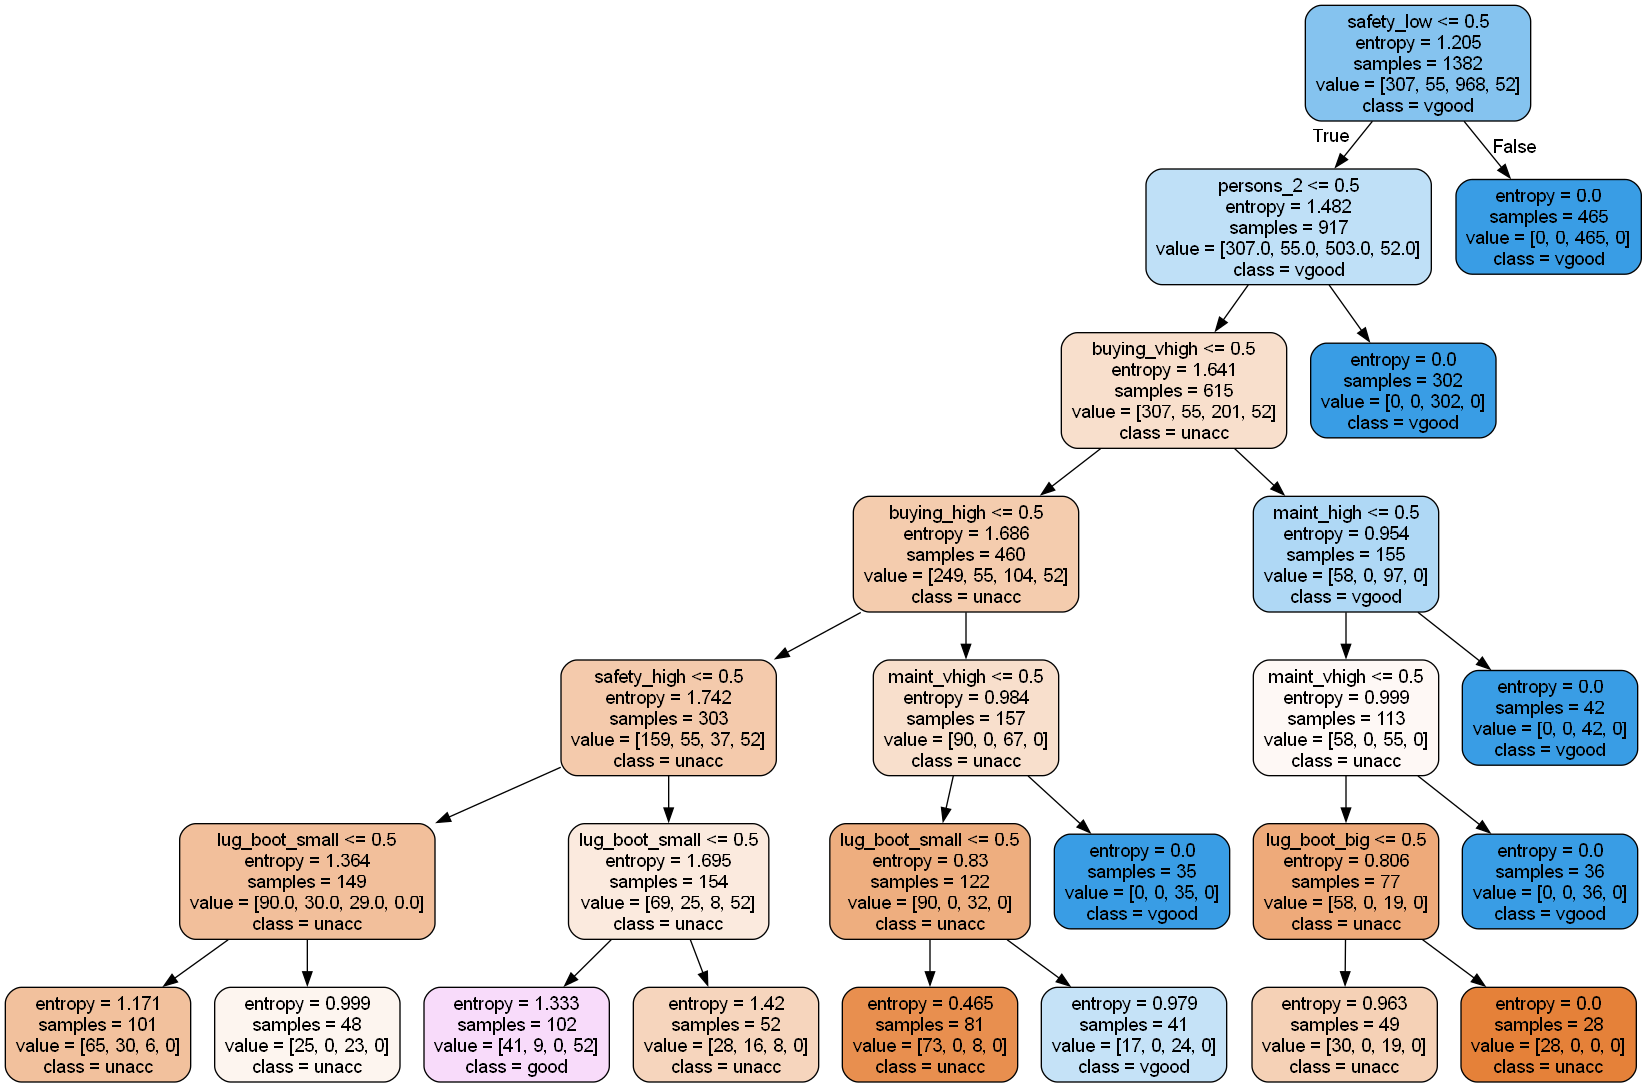
\includegraphics[width=0.8\textwidth]{imgs/dt/dt__car_evaluation__80_vs_20__6.png}
	\caption{Car Evaluation: decision tree with \texttt{max\_depth}=6 (80/20 split).}
	\label{fig:ce-dt-depth-6}
\end{figure}

\begin{figure}[H]
	\centering
	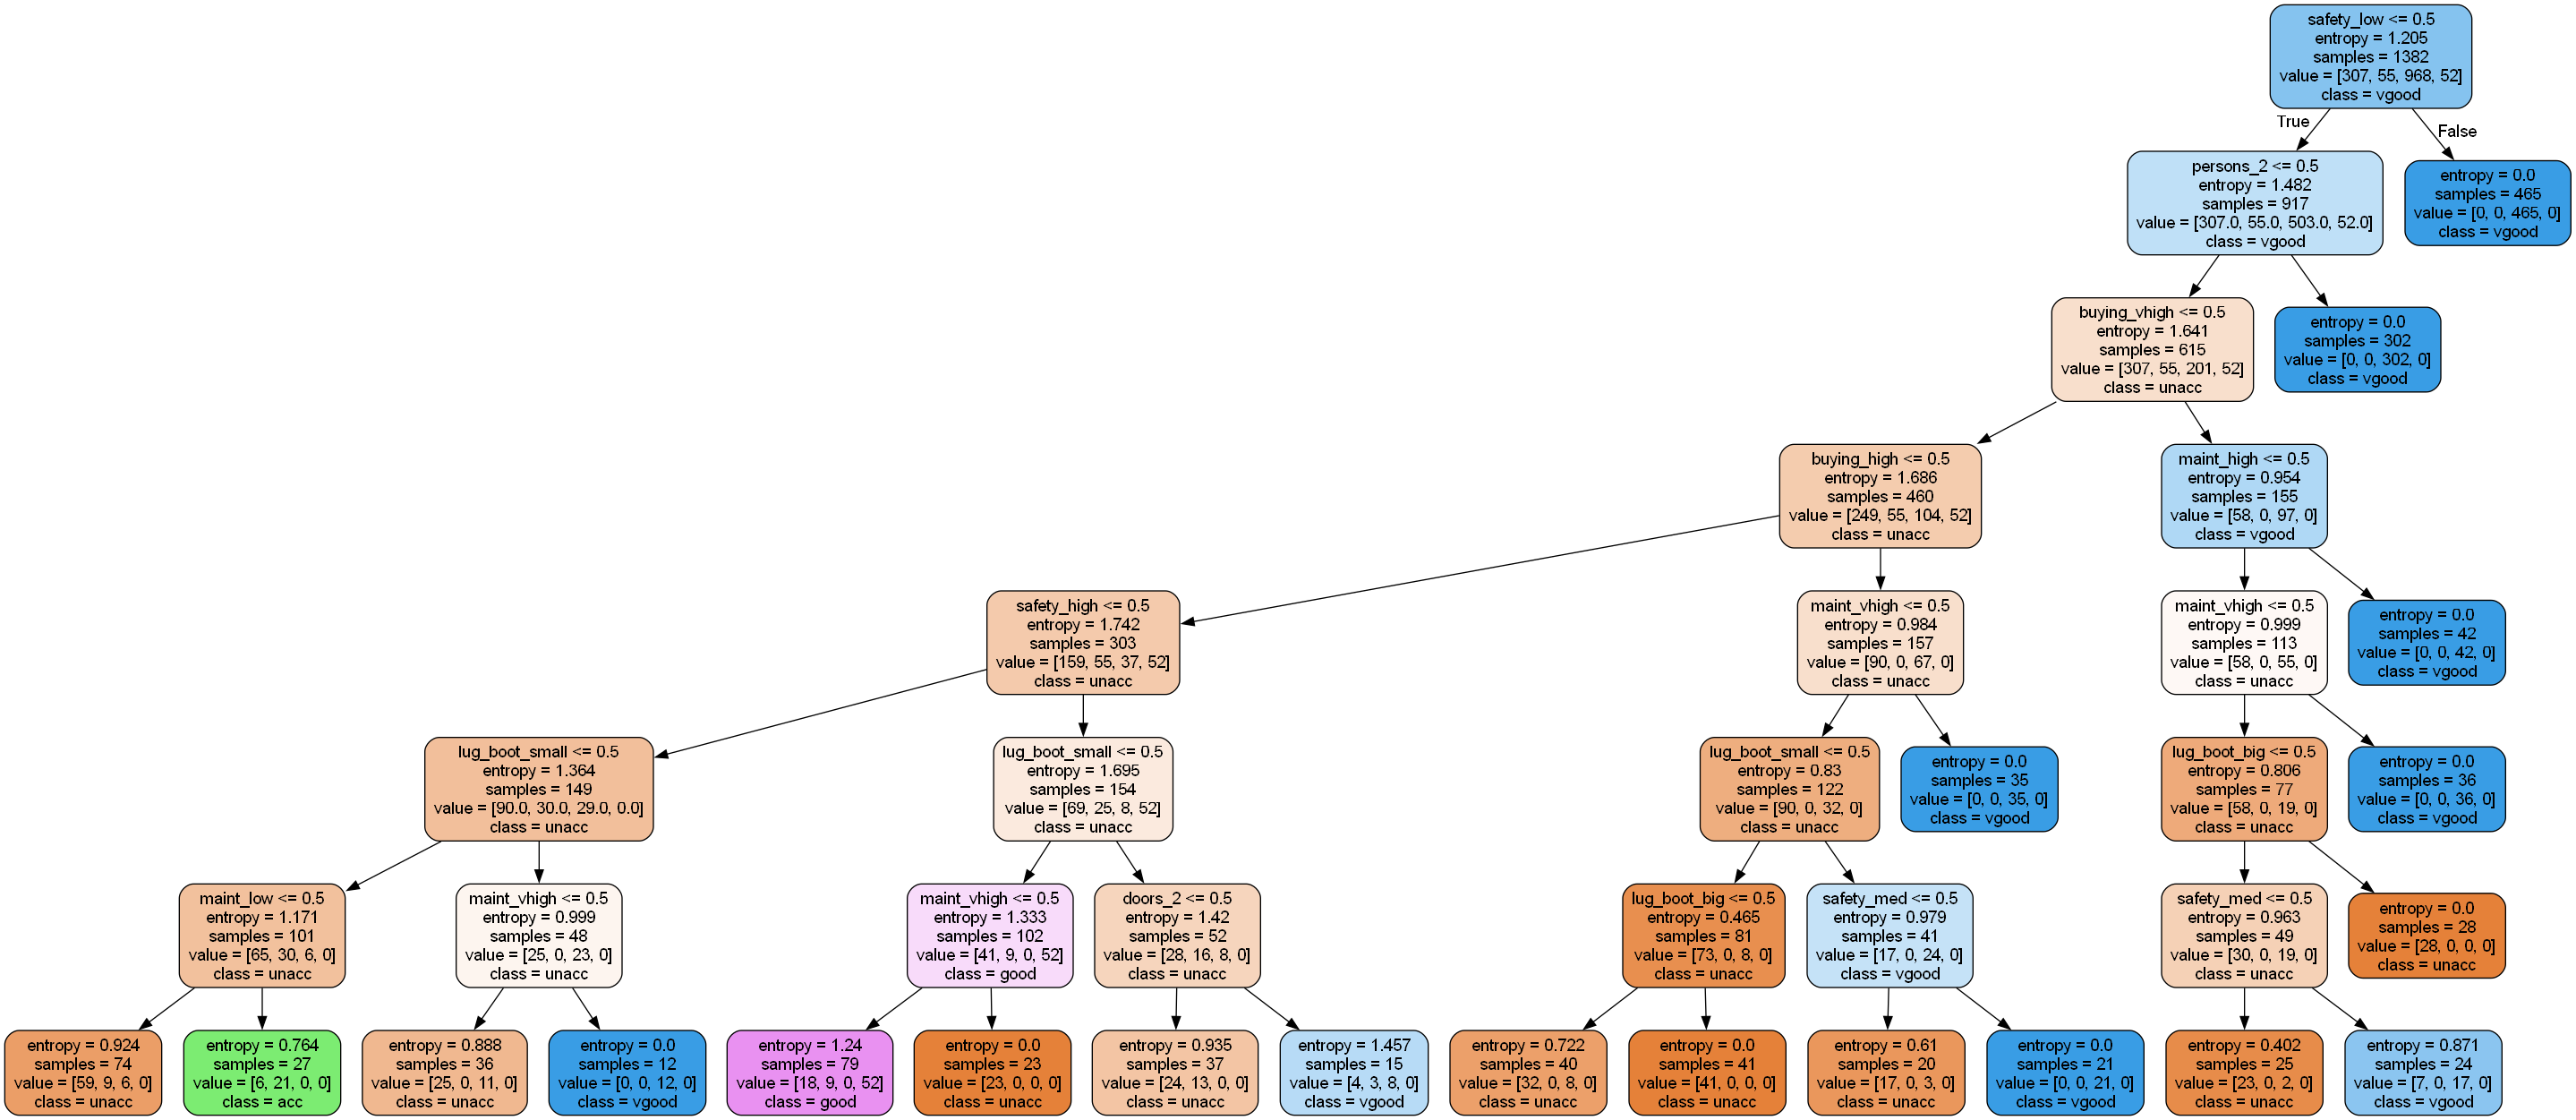
\includegraphics[width=0.8\textwidth]{imgs/dt/dt__car_evaluation__80_vs_20__7.png}
	\caption{Car Evaluation: decision tree with \texttt{max\_depth}=7 (80/20 split).}
	\label{fig:ce-dt-depth-7}
\end{figure}

\begin{figure}[H]
	\centering
	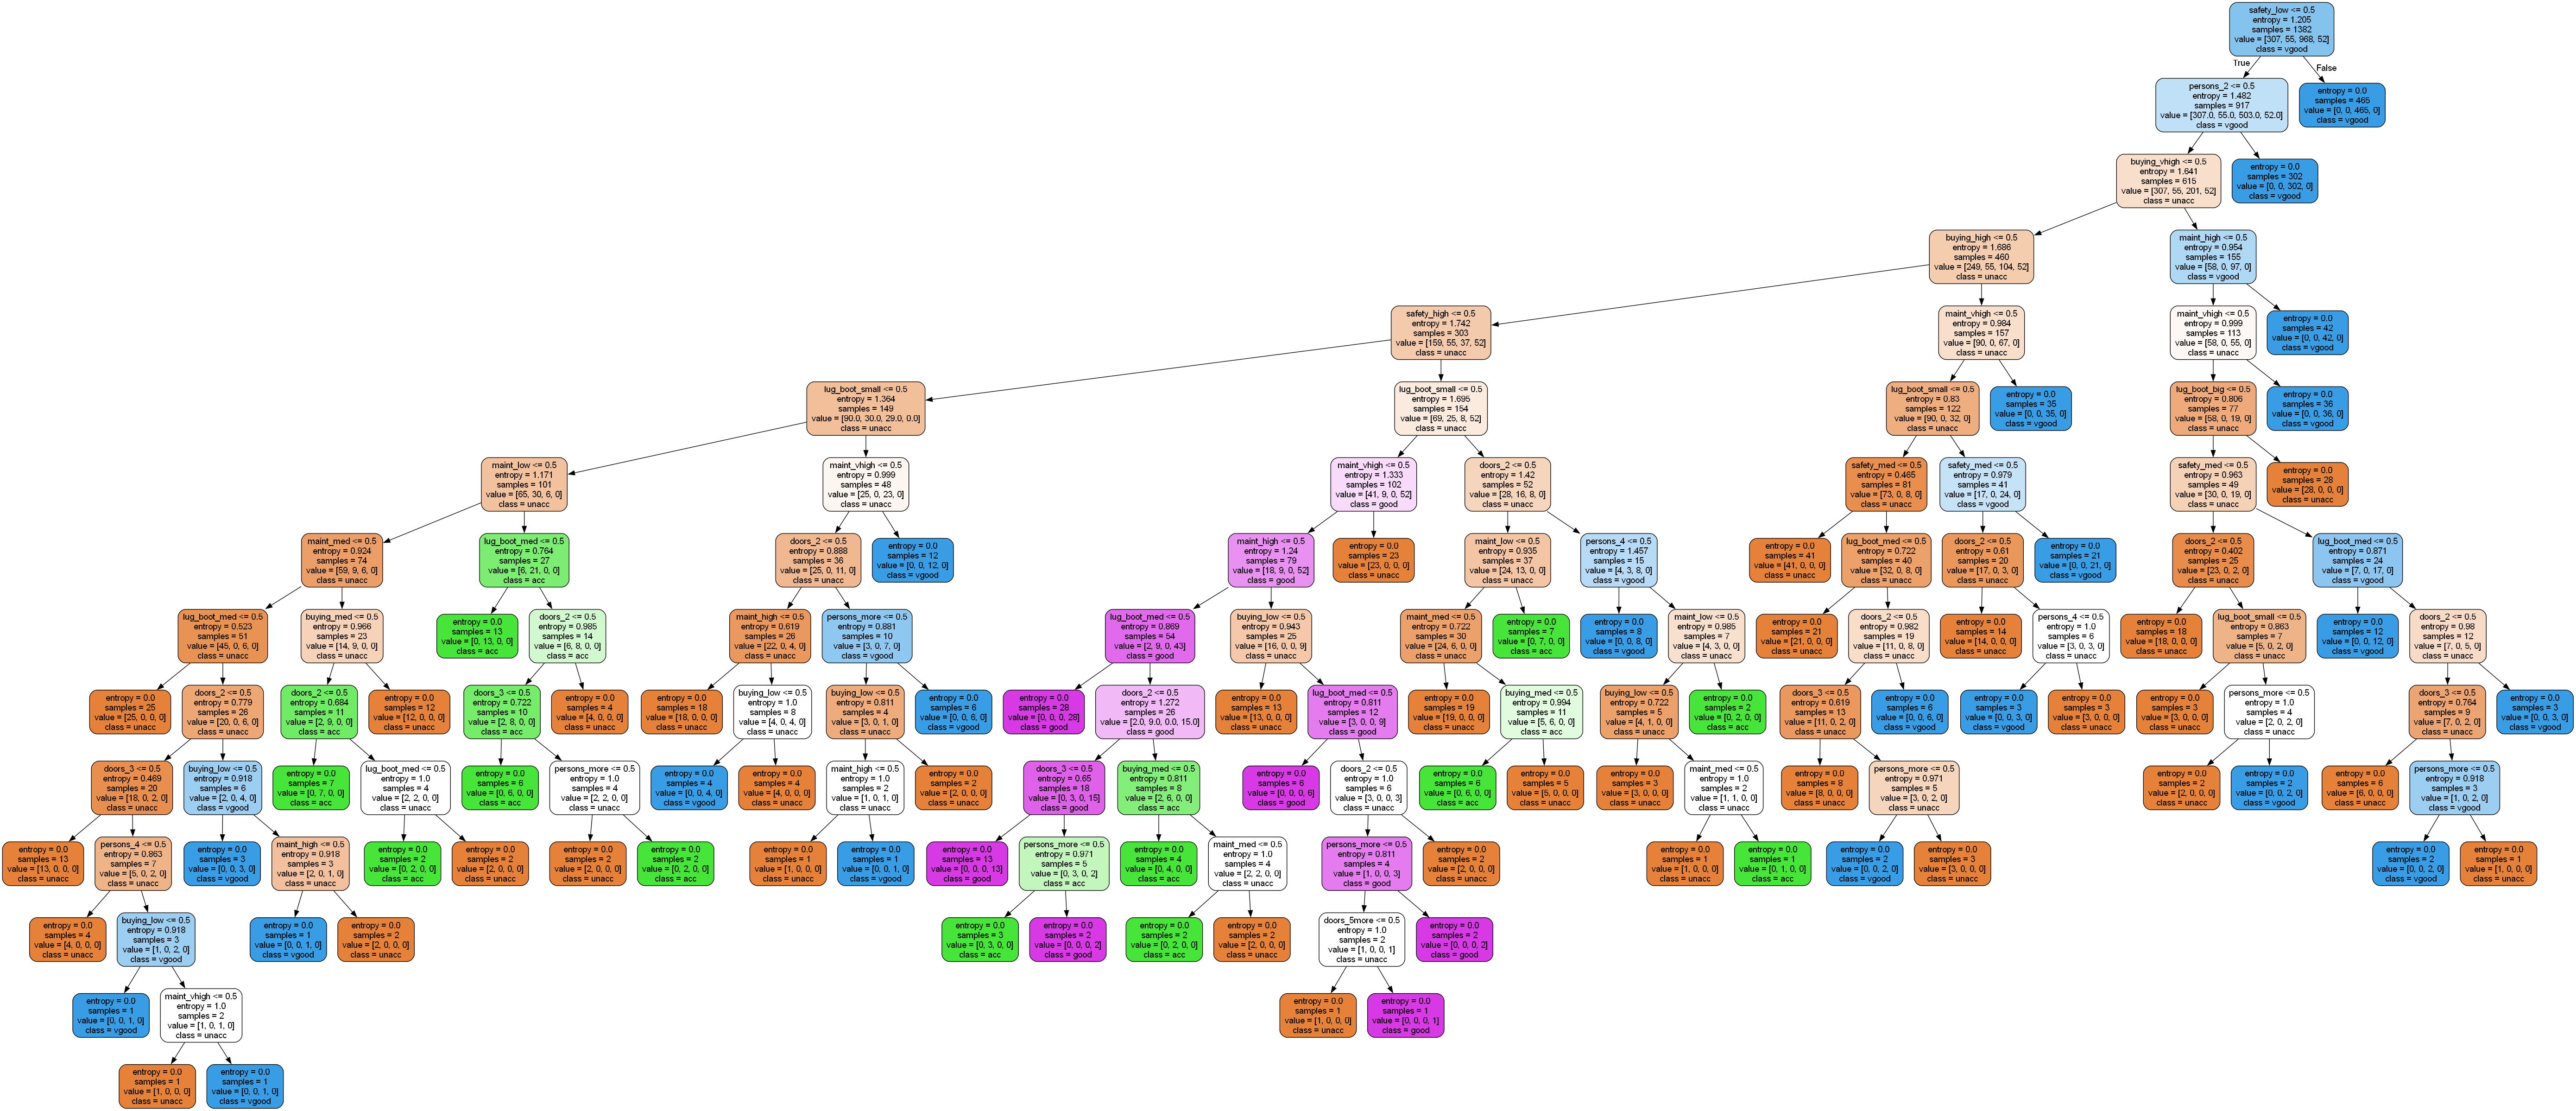
\includegraphics[width=0.8\textwidth]{imgs/dt/dt__car_evaluation__80_vs_20__None.png}
	\caption{Car Evaluation: decision tree with \texttt{max\_depth}=None (80/20 split).}
	\label{fig:ce-dt-depth-none}
\end{figure}
